\graphicspath{{./images/DBN_SS/}}
\chapter{DB-nets Analysis : State Space}
\label{ch:DBN_SS}
\paragraph*{\textnormal{In the previous chapter, we discussed how to model DB-nets in CPN Tools. In this chapter, we try to generate state space for DB-nets using CPN Tools. In the attempt for generating state spaces, we mention our few failed attempts while constructing state space using CPN Tools. In the end, we present a workaround for calculating the state space.}}
\section{State Space}
\label{sec:DBN_SS_State_Space}
\paragraph*{\textnormal{State spaces in CPN Tools can be drawn with help of the state space tool\footnote{For information about using state space tool is explained in \cite{CPN_Tools_State_Space}.}. Here, we present a more abstract version of the taxi booking example in Figure \ref{fig:DBN_SS_Faulty_Net}. In this figure, we have intentionally kept our DB-net short in order to show the full state space.}}

\begin{figure}[!htbp]
	\centering
	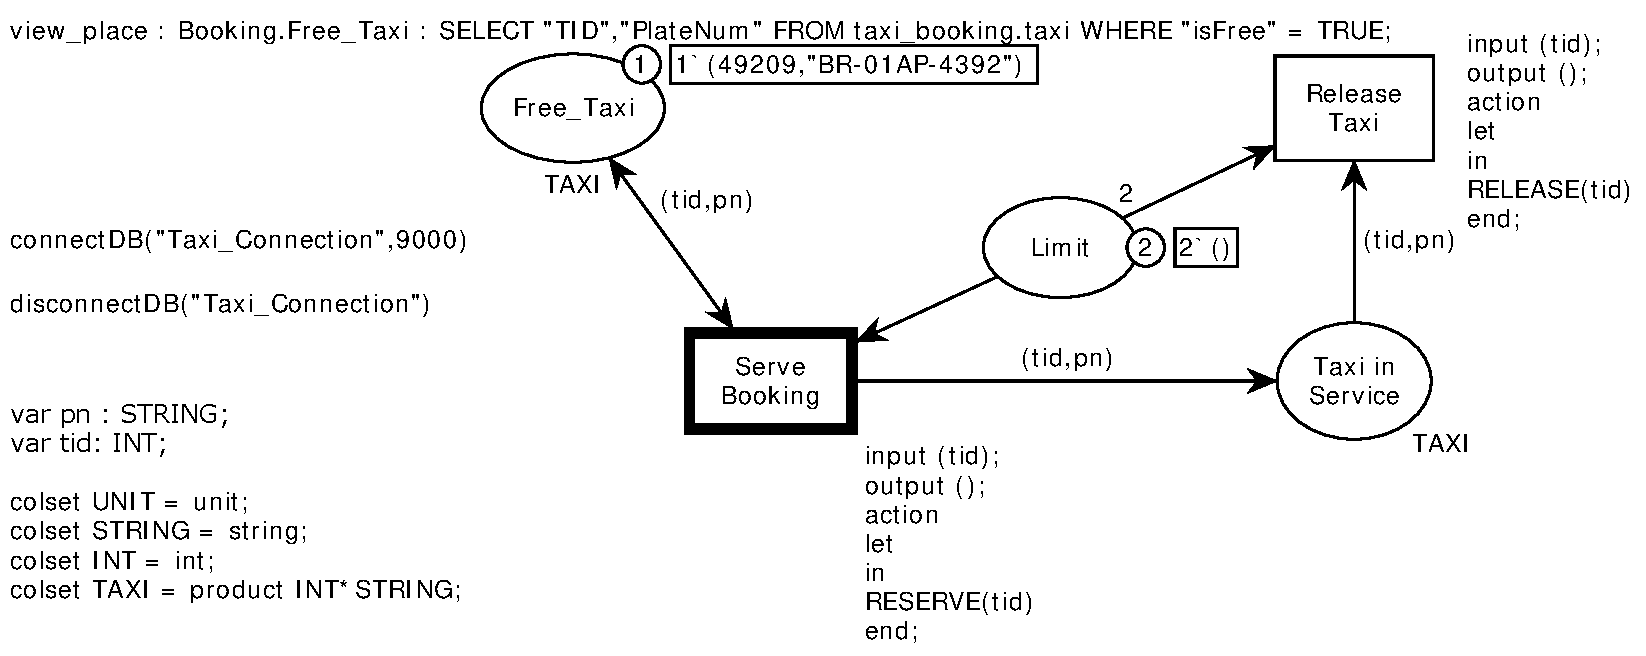
\includegraphics[scale = 0.40]{DBN_SS_Faulty_Net.pdf}
	\caption{Abstract net for taxi booking example}
	\label{fig:DBN_SS_Faulty_Net}
\end{figure}

\subparagraph*{\textnormal{In Figure \ref{fig:DBN_SS_Faulty_Net}, $\mathit{Free\_Taxi}$ is a view place(populated), $\mathit{Serve\ Booking}$ is an action transition which reserves a taxi, and makes it unavailable for further booking. Once the booking is served, the action transition $\mathit{Release\ Taxi}$ releases the taxi under service and makes it available for further booking. The place $\mathit{Limit}$ acts as the bound to the net by limiting the number of times the transitions can be fired. Here, we want to fire each transition only once. Figure \ref{fig:DBN_SS_Expected_SS} represents the expected\footnote{by \bsq{expected} we mean the ideal state space. Later we verify if we could obtain this state space using state space tool in CPN Tools.} state space for the DB-net model (Figure \ref{fig:DBN_SS_Faulty_Net}).}}

\begin{figure}[!htbp]
	\centering
	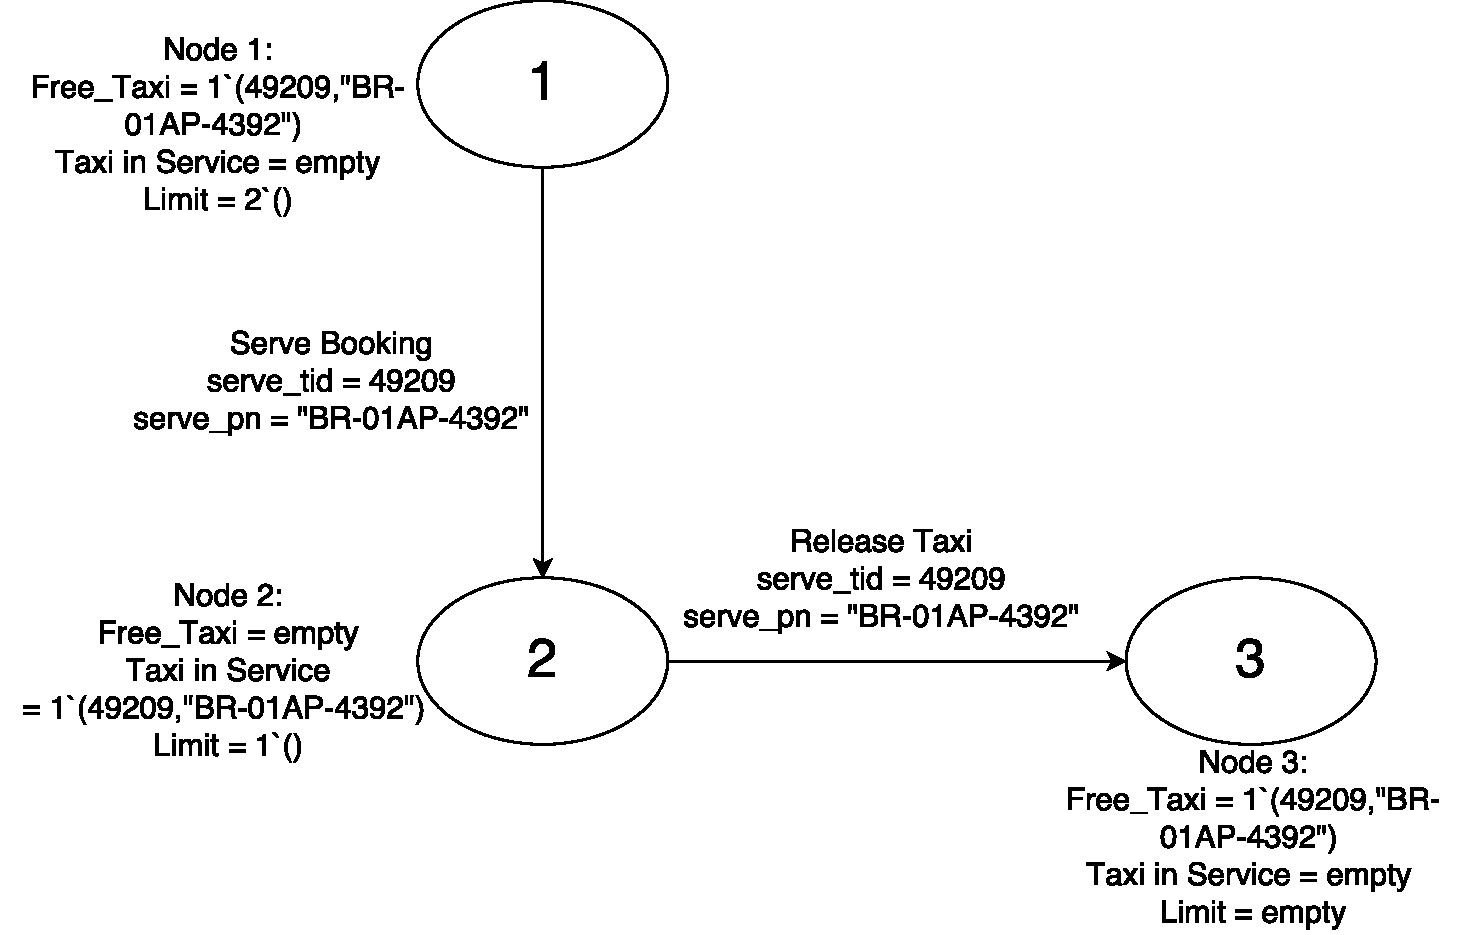
\includegraphics[scale = 0.40]{DBN_SS_Expected_State_Space.pdf}
	\caption{Expected state space for taxi booking example in Figure \ref{fig:DBN_SS_Faulty_Net}}
	\label{fig:DBN_SS_Expected_SS}
\end{figure}

\subparagraph*{\textnormal{However, when we analyse the DB-net (Figure \ref{fig:DBN_SS_Faulty_Net}) in CPN Tools, we receive the state space graph mentioned in Figure \ref{fig:DBN_SS_Faulty_Net_State_Space}. The uppermost integer in the node represents the node number whereas the numbers below it, in the format \[\langle numberofPredecessor : numberofSuccessor\rangle\] represents the number of predecessor and successor of the node. For example, node 1 has no predecessor and one successor. Similarly, node 2 has one predecessor (node 1) and two successors (node 3 and 4). The node markings are written beside the node and labels on the arcs are represented in the format \[\langle arcNumber : sourceNode \rightarrow targetNode\ transitionName : \{variableBindings\}\rangle\]For example, the directed arc between node 1 and 2 has the arc number 1, node 1 as the source node and node 2 as the target node. The transition fired is $\mathit{Booking\textquotesingle Serve\_Booking}$\footnote{It is the full qualified name of the transition, here $\mathit{Booking}$ is the page name in which the net is drawn and $\mathit{Serve\_Booking}$ is the transition name (spaces in the transition name are replaced with $\_$ symbol).} and the corresponding variable bindings are mentioned in the curly braces.}}

\subparagraph*{\textnormal{The reason for the incorrect state space calculated by CPN Tools is the inability to populate view places after firing transitions. Note that, the extension we developed is responsible for populating the view places. The state space tool in CPN Tools works as an extension and CPN Tools does not give us subscription to events occurring during state space generation\footnote{List of messages which could be subscribed by an extension are mentioned in \cite{CPN_Tools_Message_Format}.}. As a result, those events cannot be subscribed/listened by the extension and the view places are not populated.}}
\begin{figure}[!htbp]
	\centering
	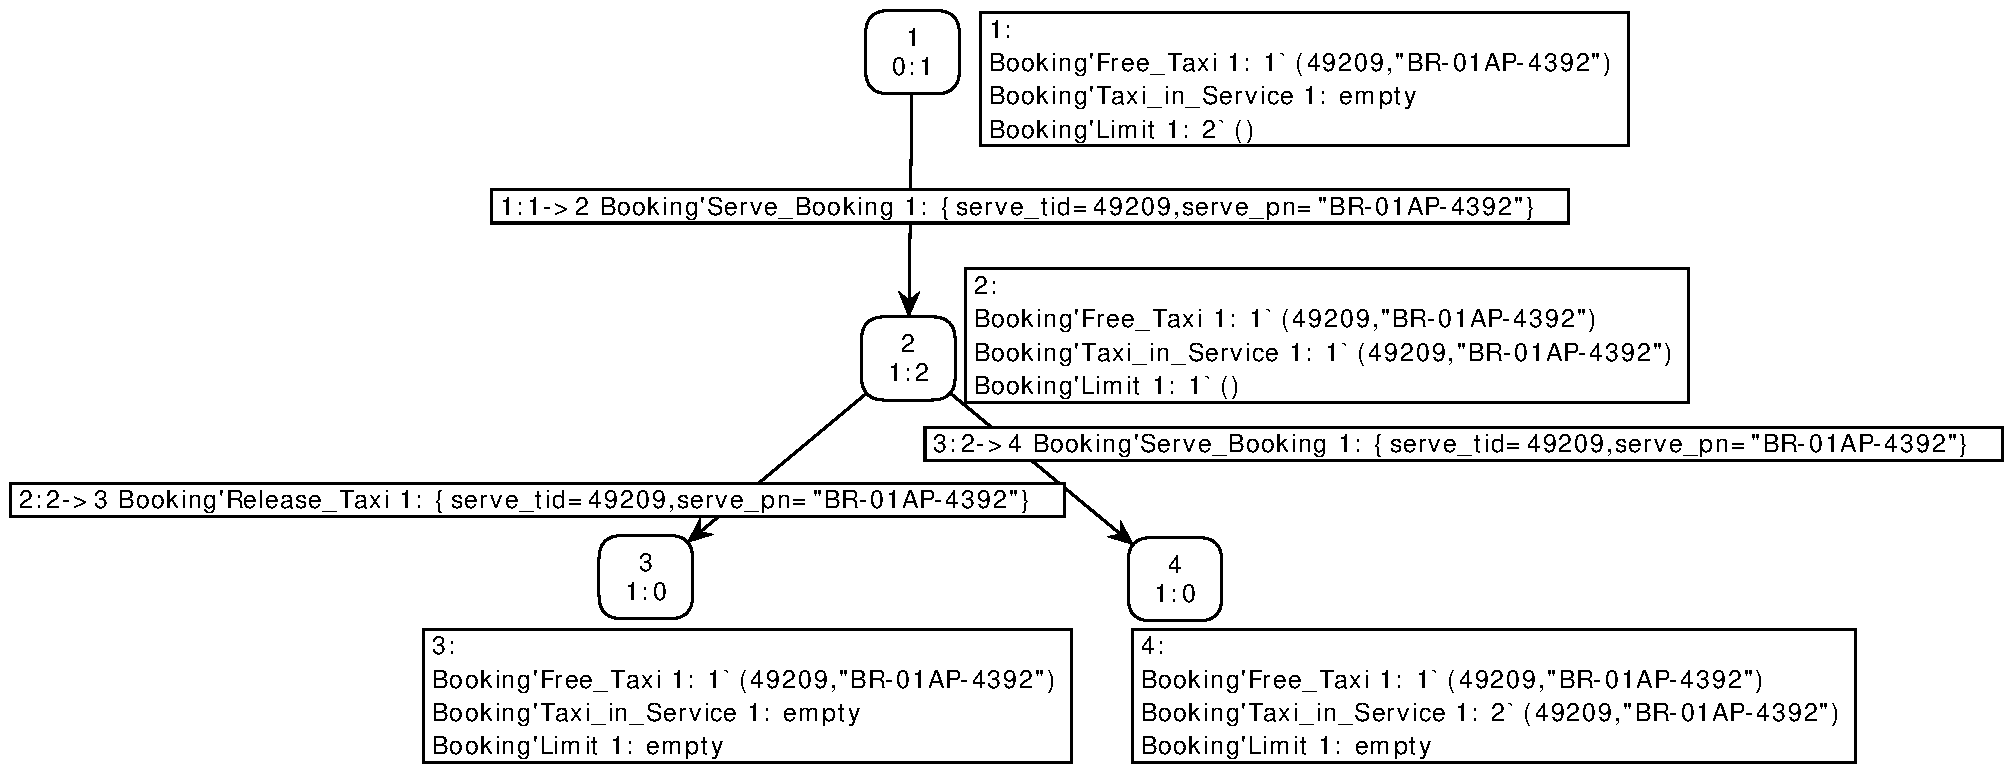
\includegraphics[scale = 0.40]{DBN_SS_Faulty_Net_State_Space.pdf}
	\caption{State Space calculated by CPN Tools for the net in Figure \ref{fig:DBN_SS_Faulty_Net}}
	\label{fig:DBN_SS_Faulty_Net_State_Space}
\end{figure}

\section{Failed Attempts}
\label{sec:DBN_SS_Failed_Attempts}
\paragraph*{\textnormal{We could successfully carry simulation over the DB-nets but we faced problem while analysing them. This section presents our failed attempts to perform analysis on DB-nets in CPN Tools. We mention our failed attempts as they are useful to understand state space generation in CPN Tools along with its relation with CPN Tools extension.}}

\subsection*{Intercepting state space construction events}
\paragraph*{\textnormal{As we mentioned earlier we could only subscribe to the events mentioned in \cite{CPN_Tools_Message_State_Space}. We tried to listen to the events which occur while drawing the state space diagram, e.g. show node marking, variable bindings of the arc etc. Once we receive the packet\footnote{The communication between GUI, simulator and extension is based on sending/receiving packets.}, we try to modify the packet by editing the node marking and replacing it with our desired marking. In the end, we return the modified packet. For example, we tried to modify the marking of node 2 (see Figure \ref{fig:DBN_SS_Faulty_Net_State_Space}) to our desired marking(by making the marking of the place $\mathit{Free\_Taxi}$ as empty). With this approach, the nodes can be modified with the desired marking, but properties such as total number of nodes (in state space), predecessor and successor needs to be changed. Even after changing the marking of the nodes, the state space report which provides the analysis of the net will yield undesired results. Intercepting state space construction events should be handled with utmost care because modifying the packet contents might lead CPN Tools into an inconsistent state, or in worst case can lead to a crash.}}

\subsection*{Shared architecture using Comms/CPN}
\paragraph*{\textnormal{We could observe that view places were not populated, but the actions in the transitions were properly executed. As mentioned, we could not capture the events, but using Comms/CPN, we could determine about the firing of the transition. We exposed a function $\mathit{refreshViewPlaces}$ from JAVA/CPN and this function was called at the end of the code segment of every transition. With this approach we created a shared architecture between the extension and JAVA/CPN as presented in Figure \ref{fig:DBN_SS_Layer_Architecture_Shared}.}}

\subparagraph*{\textnormal{In this attempt, we were successful in getting control from JAVA/CPN to the extension which was not possible in the earlier attempt. When the state space tool calculates the state space, it acquires the simulator lock and calculates its marking by firing transitions. The problem arose while updating the view place. In order to update the view place we acquire the simulator lock and send a request to GUI to update the view place. Since the simulator lock is already acquired by the state space tool, populating the view place ends up in a blocking queue where the extension waits indefinitely for the lock to get released. Since the extension is blocked, it cannot pass control to CPN Tools. Hence, we end up in an inconsistent state.}}

\begin{figure}[!htbp]
	\centering
	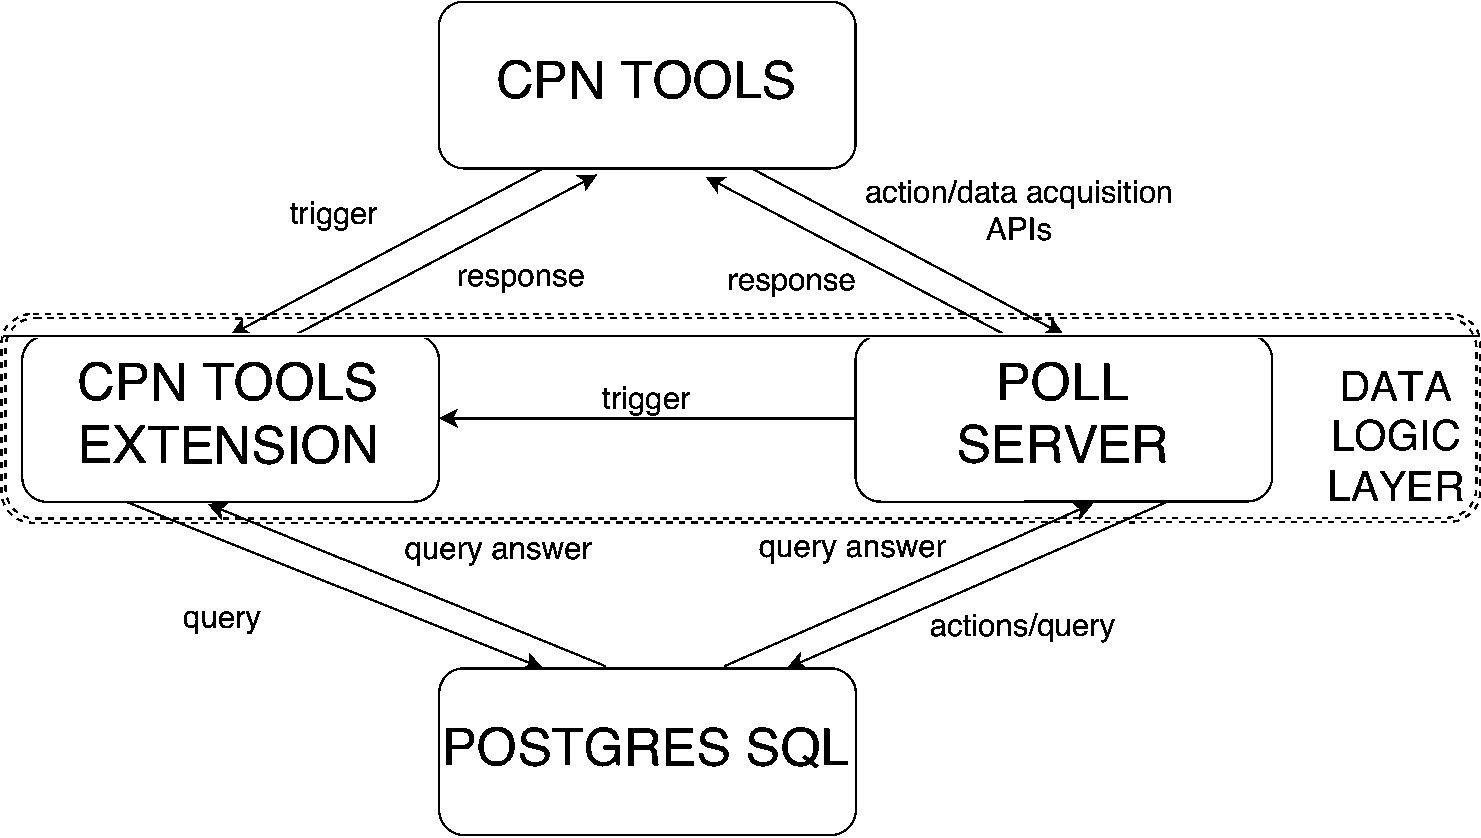
\includegraphics[scale = 0.40]{DBN_SS_Layer_Architecture_Shared.pdf}
	\caption{Shared architecture between extension and JAVA/CPN}
	\label{fig:DBN_SS_Layer_Architecture_Shared}
\end{figure}

\section{Compiling DB-nets into CPN}
\paragraph*{\textnormal{As stated earlier, the problem is to populate view places through the extension during state space calculation, hence we try to populate them through the net elements. Instead of relying on the database, we project the contents of the database on the control layer, and update the contents using net elements. In this approach, instead of view places we model \textit{relational places}. \textit{Relational places} are places which project the contents of the relational schema and the tokens in the relational places show the instances of the corresponding relational schema. The place colour mirrors the components of the relation schema and their types. In this light, each token represents a tuple in the database. Thus, with this approach we lift the database schema and model it in our control layer.  Later, we try to manually update the marking of the relational places by removing and/or inserting tokens corresponding to the actions attached to the transitions. In this workaround, the database is considered to be without any constraints. However, the proposed solution can seamlessly account for constraints as well.}}

\paragraph*{\textnormal{Before we introduce the modelling of relational places, we introduce \textit{priority} of a transition \cite{DBLP:conf/apn/WestergaardV11}. One can give high priority to a transition to force it to occur before all other enabled transitions, which can be used in case of exception handling by prioritizing the exception handler over other transitions handling usual cases. Similarly, one can assign lower priority to transition to prevent it from occurring unless no other transitions are enabled. As mentioned in \cite{CPN_Tools_Priority_Transitions}, in CPN Tools, we can assign priority to each transition. A \textit{priority} is simply a predefined integer\footnote{higher the value of integer, lower is the priority.} attached to a transition. If the priority of a transition is not explicitly defined, then it is considered as a \textit{NORMAL} priority transition. One can also define custom priorities in CPN Tools. In our case, we declare priority values as:
}}
\begin{verbatim}
val P_HIGH = 100;
val P_NORMAL = 1000;
val P_LOW = 10000;
\end{verbatim}}}

\subsection{View Place computation using Relational Places}
\label{subsec:DBN_SS_view_place_computation}

\subparagraph*{\textnormal{Let us consider a database schema \textit{organisation} containing the relational schema \textit{emp}, \textit{empDescr} and \textit{empID} as shown in Figure \ref{fig:DBN_SS_Relational_Schema}. The \textit{emp} table contains the id of the employee, name of the employee, and busy status of the employee. Table \textit{empDescr}\footnote{a short name for employee description.} contains the name of employees along with their designation and the table \textit{empID} contains the employee id. We use this database schema for modelling DB-net examples which are later transformed into CPNs.
\begin{figure}[!htbp]
	\centering
	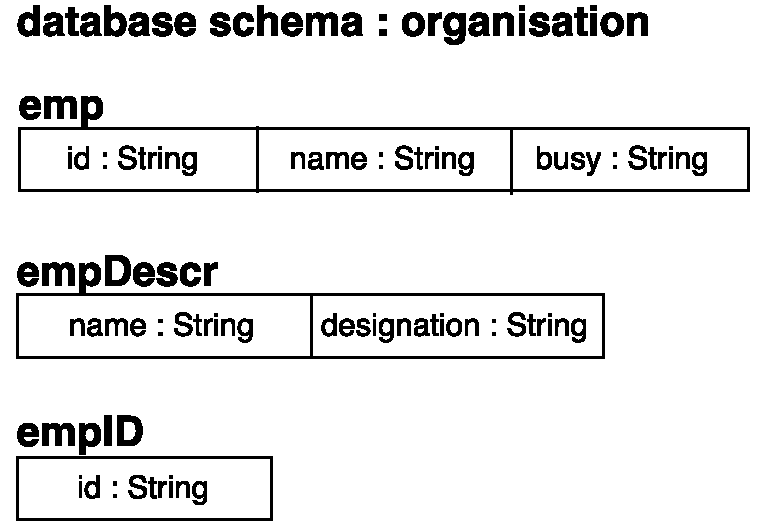
\includegraphics[scale = 0.50]{DBN_SS_Relational_Schema.pdf}
	\caption{Database Schema : organisation}
	\label{fig:DBN_SS_Relational_Schema}
\end{figure}
}}

\paragraph*{\textnormal{A small DB-net example is shown in Figure \ref{fig:DBN_SS_View_Place_1}, where we obtain a salary for a designation. The designation is computed using the \textit{View Place} and the query attached to it is:
\begin{figure}[h]
	\centering
	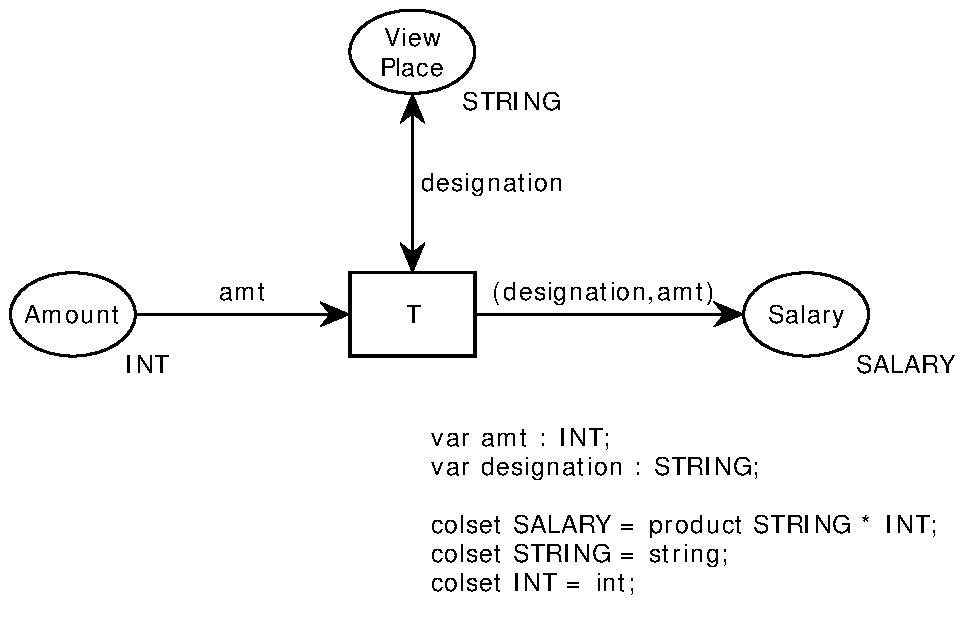
\includegraphics[scale = 0.50]{DBN_SS_View_Place_1.pdf}
	\caption{DB-nets: one view place}
	\label{fig:DBN_SS_View_Place_1}
\end{figure}}}

\subparagraph*{}
\begin{lstlisting}[showstringspaces=false, language = SQL]
SELECT organisation.empDescr.designation FROM organisation.empDescr, organisation.emp WHERE organisation.empDescr.name = organisation.emp.name;
\end{lstlisting}

\subparagraph*{\textnormal{Once	we have relational places, then we can compile away view places by reconstructing their content via a suitable query over relational places. Such a query can be formulated directly using arcs and inscriptions of the net, i.e., by resorting to standard elements in CPNs. Since, all queries attached to view places could not be evaluated using relational places, we restrict ourselves to conjunctive queries with filters. The filter condition in the conjunctive queries, attached to the view places, can be modelled using guards of the transition. For example, in Figure \ref{fig:DBN_SS_Relational_Place_1}, the relational places are modelled using places \textit{emp} and \textit{empDescr} projecting the contents of the corresponding relational schemas. The guard on the transition incorporates the filter condition.}}
\begin{figure}[h]
	\centering
	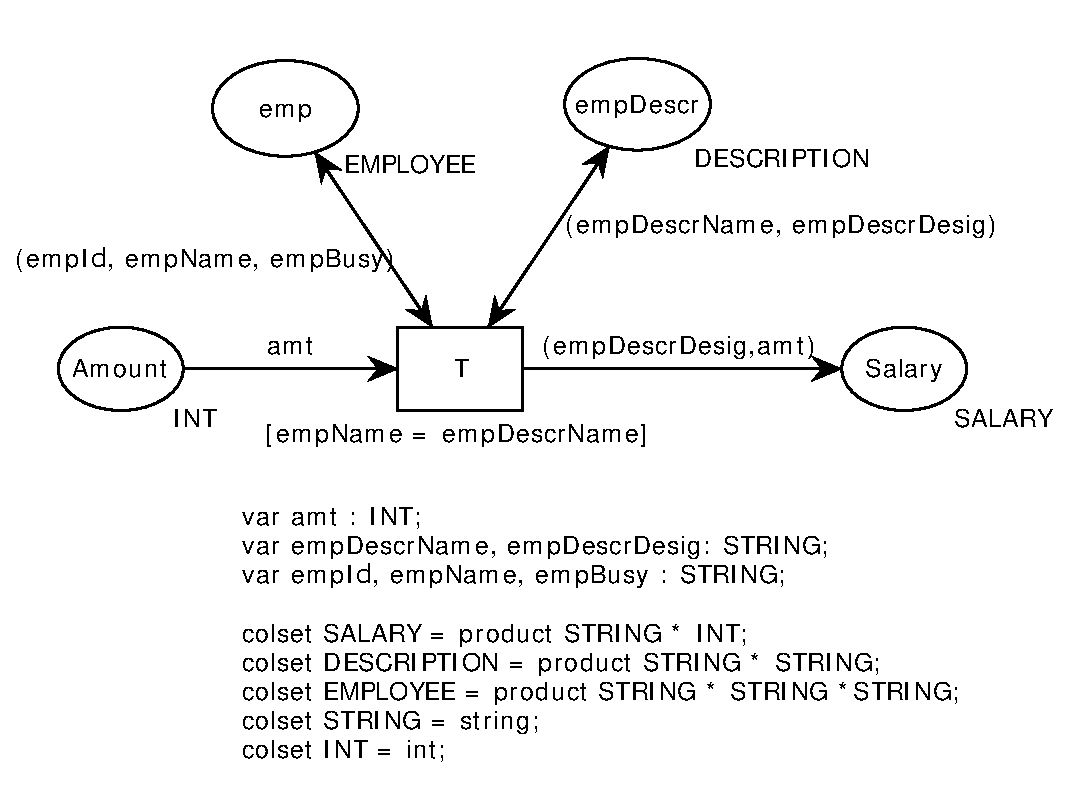
\includegraphics[scale = 0.50]{DBN_SS_Relational_Place_1.pdf}
	\caption{DB-nets: computing a view place using relational places}
	\label{fig:DBN_SS_Relational_Place_1}
\end{figure}

\subparagraph*{\textnormal{In case there are multiple view places sharing one or more relational schemas, the contents of the view place can be calculated in a sequential manner. Using a separate transition, we generate tokens of the first view place and then the generated tokens are forwarded to another transition which generates marking for the second view place. Similarly, in a serialized pipeline, one could calculate the result of two view places, and pass the result for calculation of third view place and so on. Let us consider an example of a transition connected to two view places as shown in Figure \ref{fig:DBN_SS_View_Place_2}. The query attached to the \textit{View Place 1} is same as the query attached to the \textit{View Place} in Figure \ref{fig:DBN_SS_View_Place_1}. The query attached to \textit{View Place 2} is:
\begin{figure}[!htbp]
	\centering
	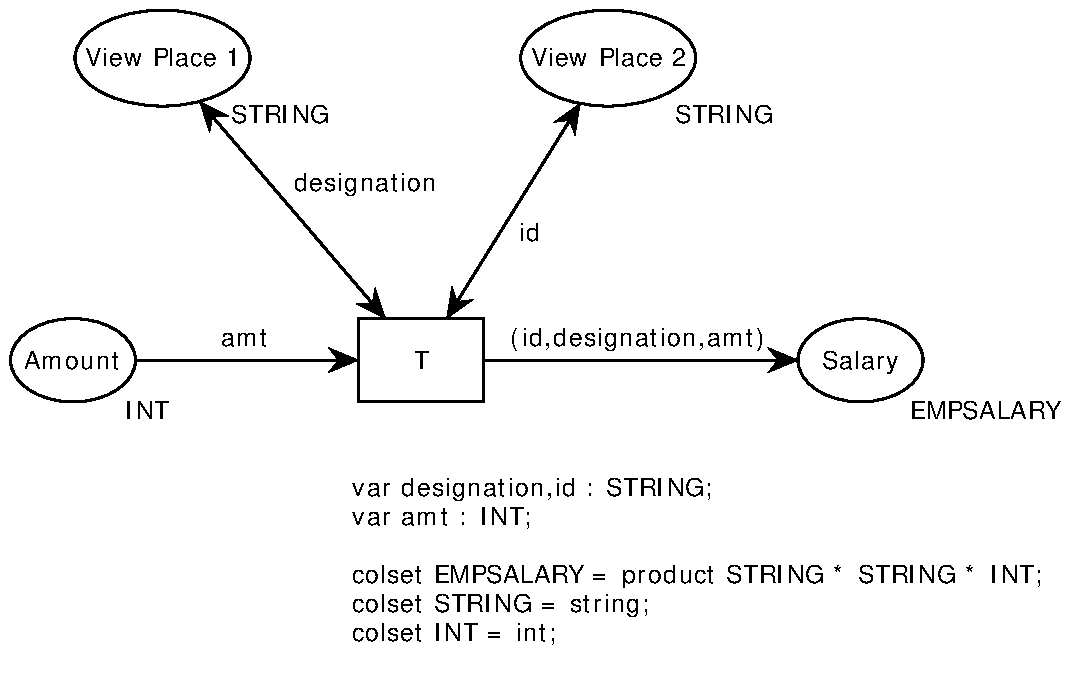
\includegraphics[scale = 0.50]{DBN_SS_View_Place_2.pdf}
	\caption{DB-nets: two view places}
	\label{fig:DBN_SS_View_Place_2}
\end{figure}
}}

\subparagraph*{}
\begin{lstlisting}[showstringspaces=false, language = SQL]
SELECT organisation.empID.id FROM organisation.empID, organisation.emp WHERE organisation.empID.id = organisation.emp.id;
\end{lstlisting}

\subparagraph*{\textnormal{The two view places use the common relational schema \textit{emp} to compute their markings. Using relational places, we could model the above net as shown in Figure \ref{fig:DBN_SS_Relational_Place_2}. In the figure, the transition \textit{Calculate View Place 1} acquires a lock (an uncoloured token) and generates a token for \textit{View Place 1} (see Figure \ref{fig:DBN_SS_View_Place_2}) which is stored at the place \textit{Result 1}. The transition $\mathit{T}$ has a higher priority (defined by the priority P\_HIGH) over the transition \textit{Release Lock}. If the transition \textit{T} is not enabled, then transition \textit{Release Lock} consumes the token from the place \textit{Result 1} and returns the lock. The purpose of lock is to allow the computation of each view place without any interruptions. Similarly, this sequential pipeline can be adopted if we have more than two view places which share a common relational schema.}}

\begin{figure}[!htbp]
	\centering
	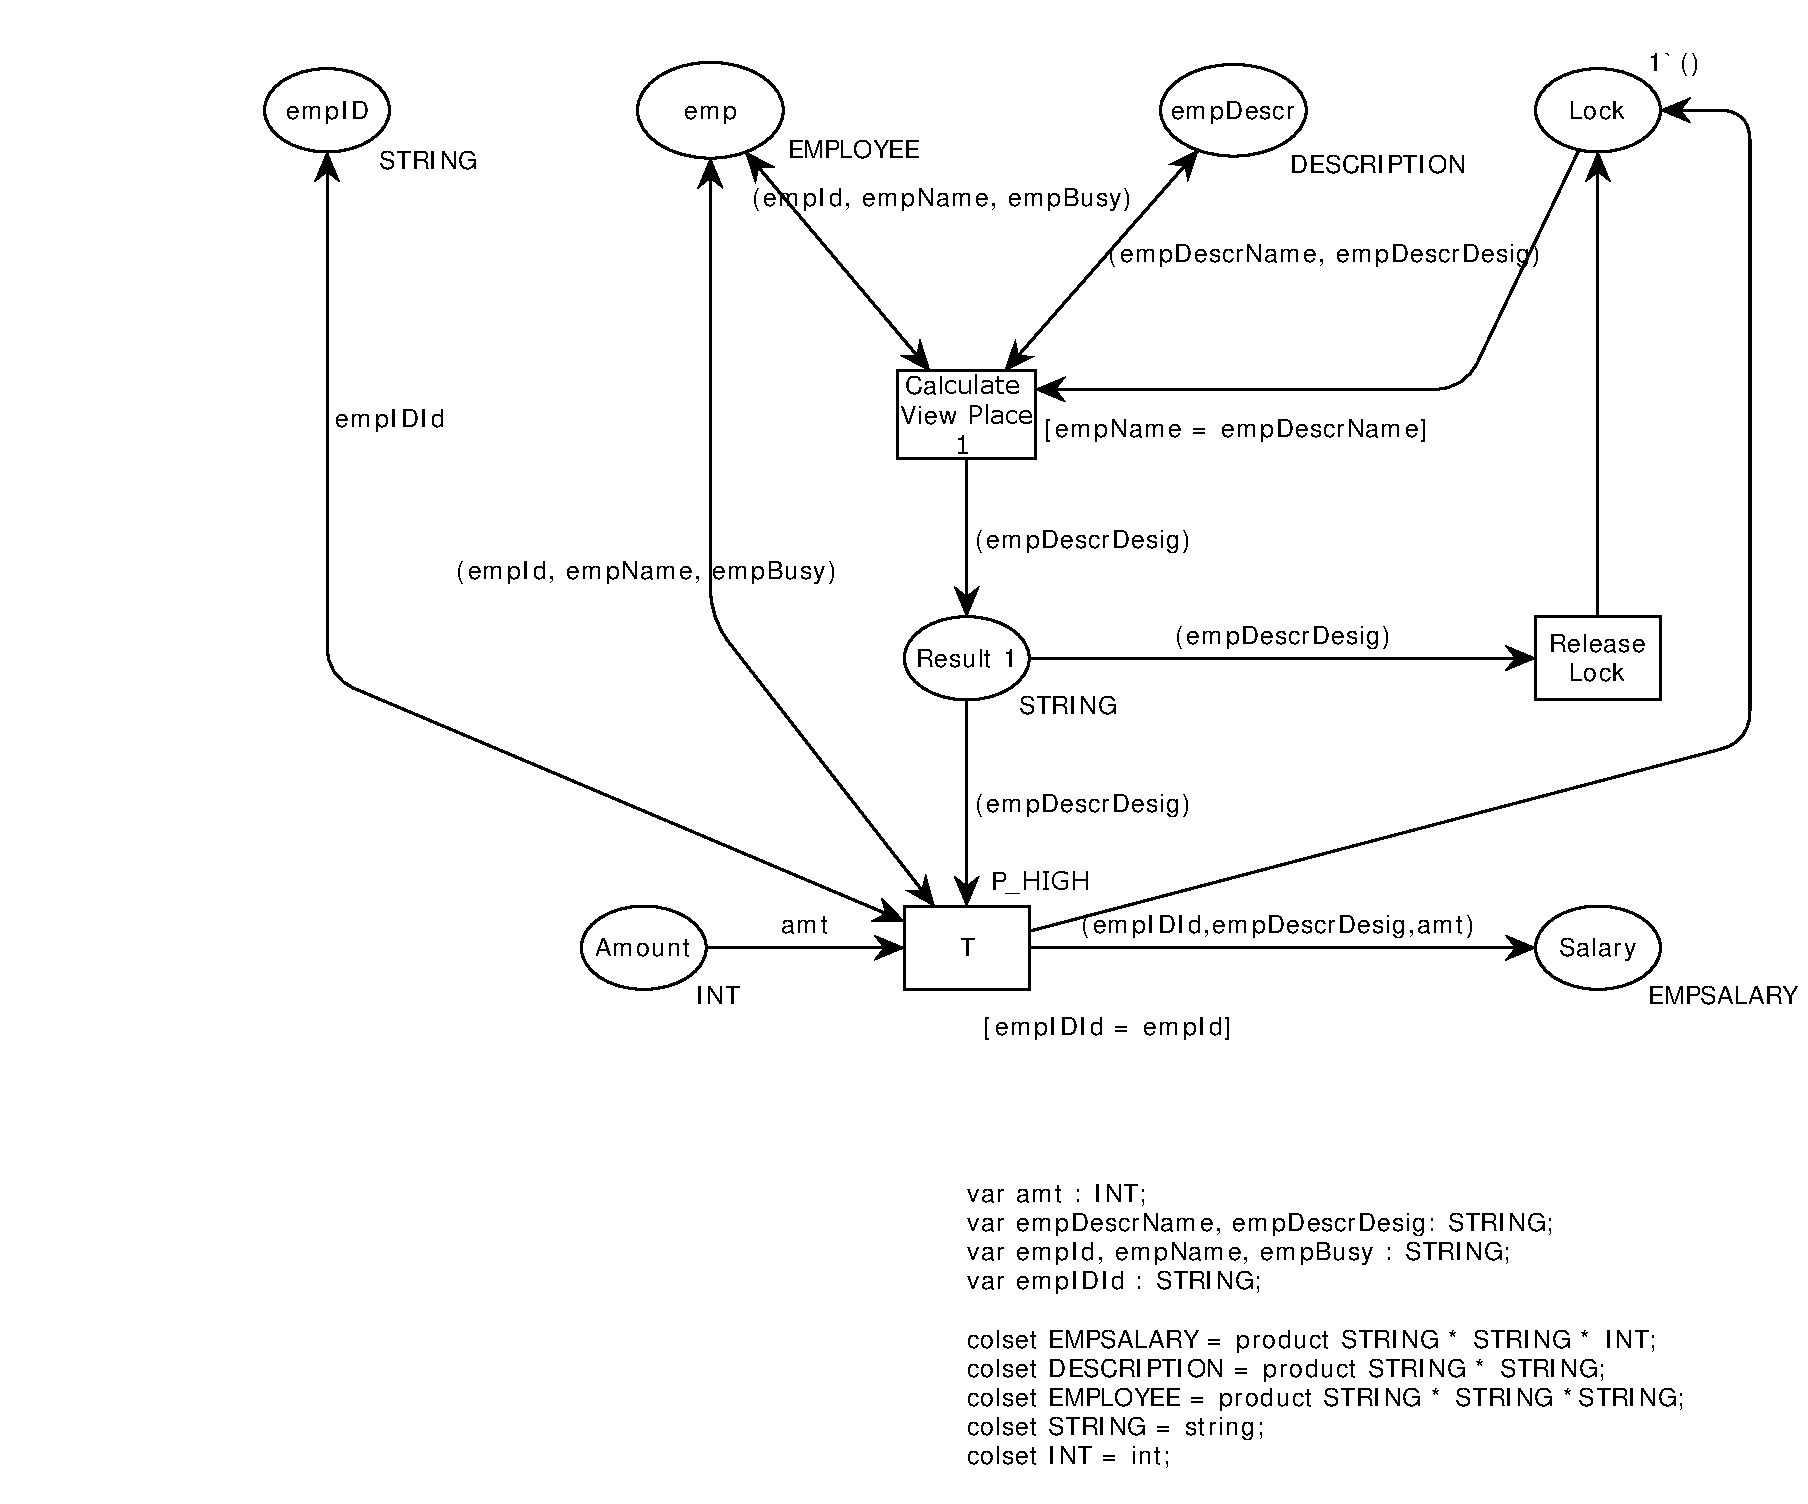
\includegraphics[scale = 0.40]{DBN_SS_Relational_Place_2.pdf}
	\caption{DB-nets: computing two view places using relational places}
	\label{fig:DBN_SS_Relational_Place_2}
	
\subparagraph*{\textnormal{Note that the $\mathit{READ}$ operation in DB-nets is modelled using view places. View places give us the partial information from the database instance whereas using relational places we represent the entire database instance. We can calculate the partial information (shown by view place) from the relational places and hence we do not need to explicitly model the read operation.}}
\end{figure}

\subsection{Transformation of Action Transitions}
\label{subsec:DBN_SS_Transformation_Action_Transitions}
\paragraph*{\textnormal{In the previous subsection, we discussed how to replace view places with relational places. In this subsection, we discuss about modelling the actions attached to a transition. In order to write into the database, we need to understand how to simulate actions over relational places. For further discussions, we use the DB-net modelled in Figure \ref{fig:DBN_SS_View_Place_1} and attach actions to the transition $\mathit{T}$.}}

\subparagraph*{\textnormal{As stated earlier, action transitions support addition and deletion of $\mathit{\mathcal{R}}$-facts, which should preserve the set semantics incorporated while modelling our persistence layer. In this workaround, the persistence layer is considered to be without any constraints. When we transform the operations, the action transition acquires the write lock before firing and releases the write lock when all the operations are executed. Figure \ref{fig:DBN_SS_Add_Operation} shows a DB-net with one transition that has an action attached which, in turn, adds a single entry to the $\mathit{empDescr}$ relational schema. In Figure \ref{fig:DBN_SS_Add_Operation_Relational_Place}, we model the net using relational places and reflect the effect of the add operation to the concerned relational place, i.e., $\mathit{empDescr}$.
\begin{figure}[!htbp]
	\centering
	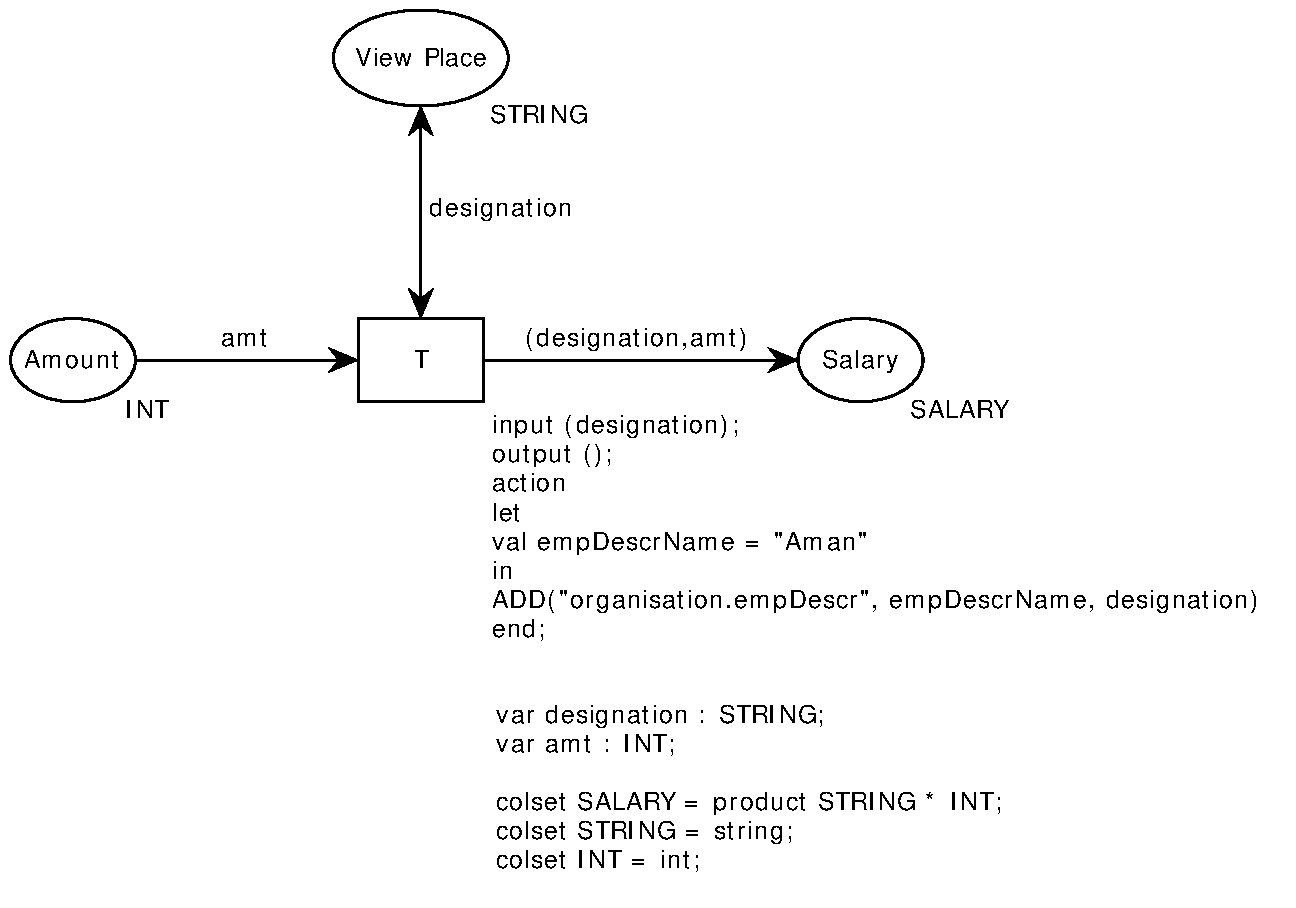
\includegraphics[scale = 0.40]{DBN_SS_Add_Operation.pdf}
	\caption{DB-nets: add operation}
	\label{fig:DBN_SS_Add_Operation}
\end{figure}
}}

\subparagraph*{\textnormal{In Figure \ref{fig:DBN_SS_Add_Operation_Relational_Place}, the transition $\mathit{T}$ acquires the \textit{write lock} (an uncoloured token) before firing. A \textit{write lock} is the lock which is acquired by an action transition to execute its action in a serialized manner. The tokens to be added are forwarded to the place $\mathit{toAdd}$. For preserving the set semantics over the relational place, with the help of priorities on the transitions, we first check if the entry already exists in the relational place. Note that the transition \bsq{$\mathit{exists\ in\ empDescr}$} has a higher priority than the transition \bsq{$\mathit{not\ exists\ in\ empDescr}$}. If the entry exists, then by firing \bsq{$\mathit{exists\ in\ empDescr}$} transition we do not add the token to the relational place, else we fire \bsq{$\mathit{not\ exists\ in\ empDescr}$} transition which adds a token to the relational place. After performing the add operation the write lock is returned.
\begin{figure}[!htbp]
	\centering
	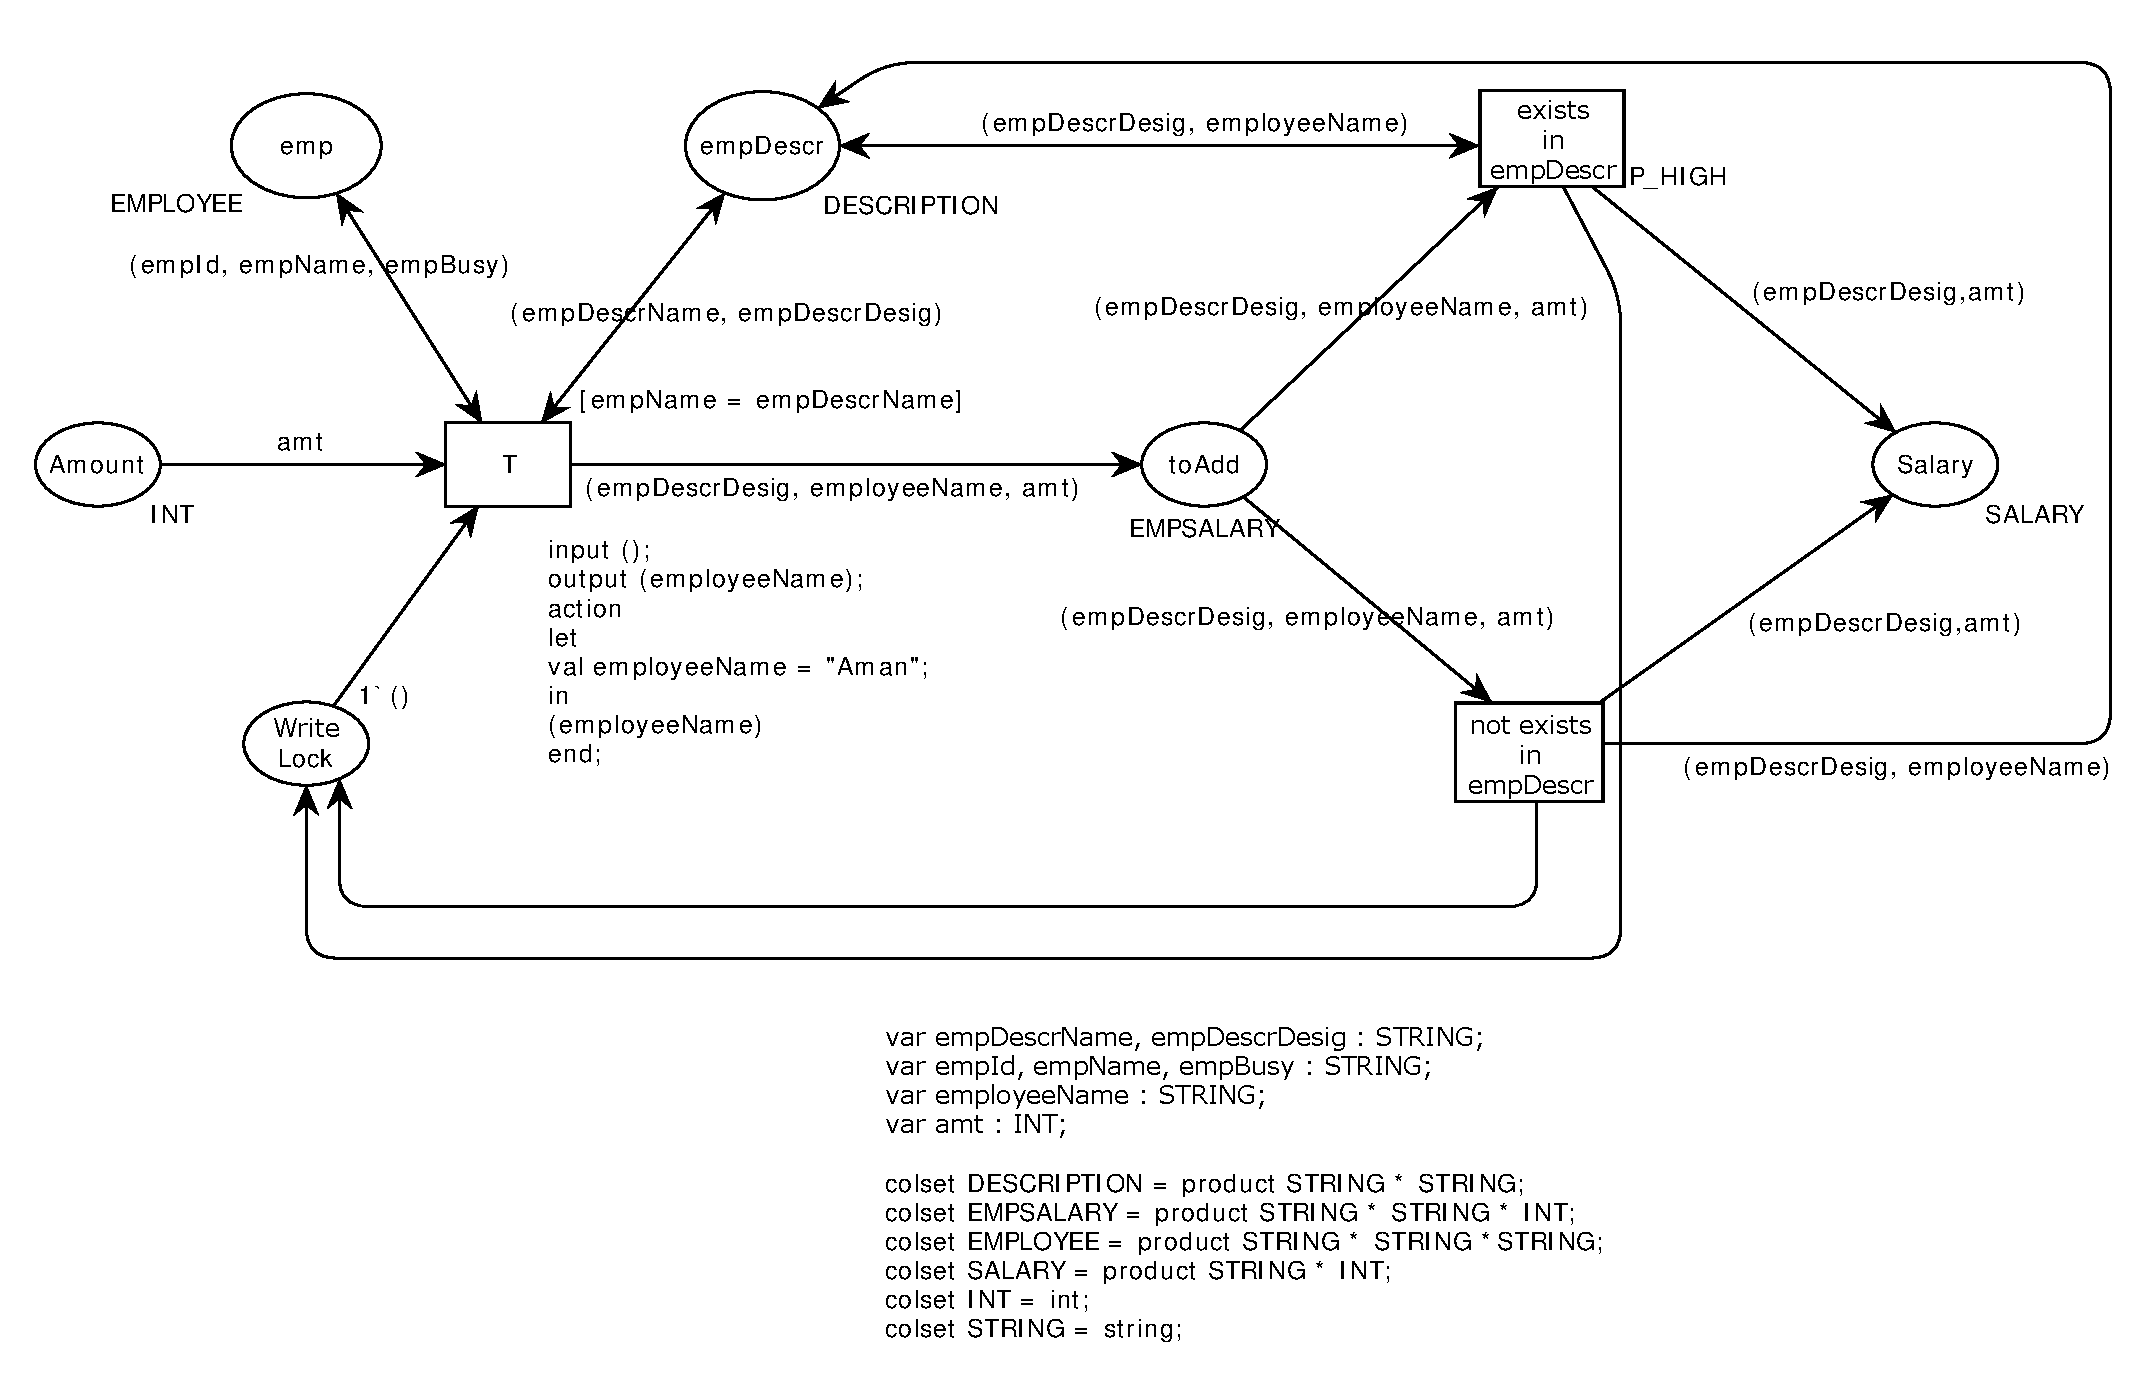
\includegraphics[scale = 0.40]{DBN_SS_Add_Operation_Relational_Place.pdf}
	\caption{DB-nets: modelling add operation using relational places}
	\label{fig:DBN_SS_Add_Operation_Relational_Place}
\end{figure}
}}

\subparagraph*{\textnormal{Similarly, we can model the $\mathit{DELETE}$ operation. Let us consider the DB-net in Figure \ref{fig:DBN_SS_Delete_Operation}, where we perform a delete operation (attached to the transition $\mathit{T}$) on the relation schema \textit{empDescr}. The corresponding transformation of the DB-net is shown in Figure \ref{fig:DBN_SS_Delete_Operation_Relational_Place} where we reflect the delete operation in the relational place $\mathit{empDescr}$. Using priority between the transitions, we first check whether the token to be deleted exists in the relational place. If the token is present in the relational place, then we fire the transition $\mathit{exists\ in\ empDescr}$ and remove the token from the relational place, else we fire the transition \bsq{$\mathit{not\ exists\ in\ empDescr}$} and proceed.
\begin{figure}[!htbp]
	\centering
	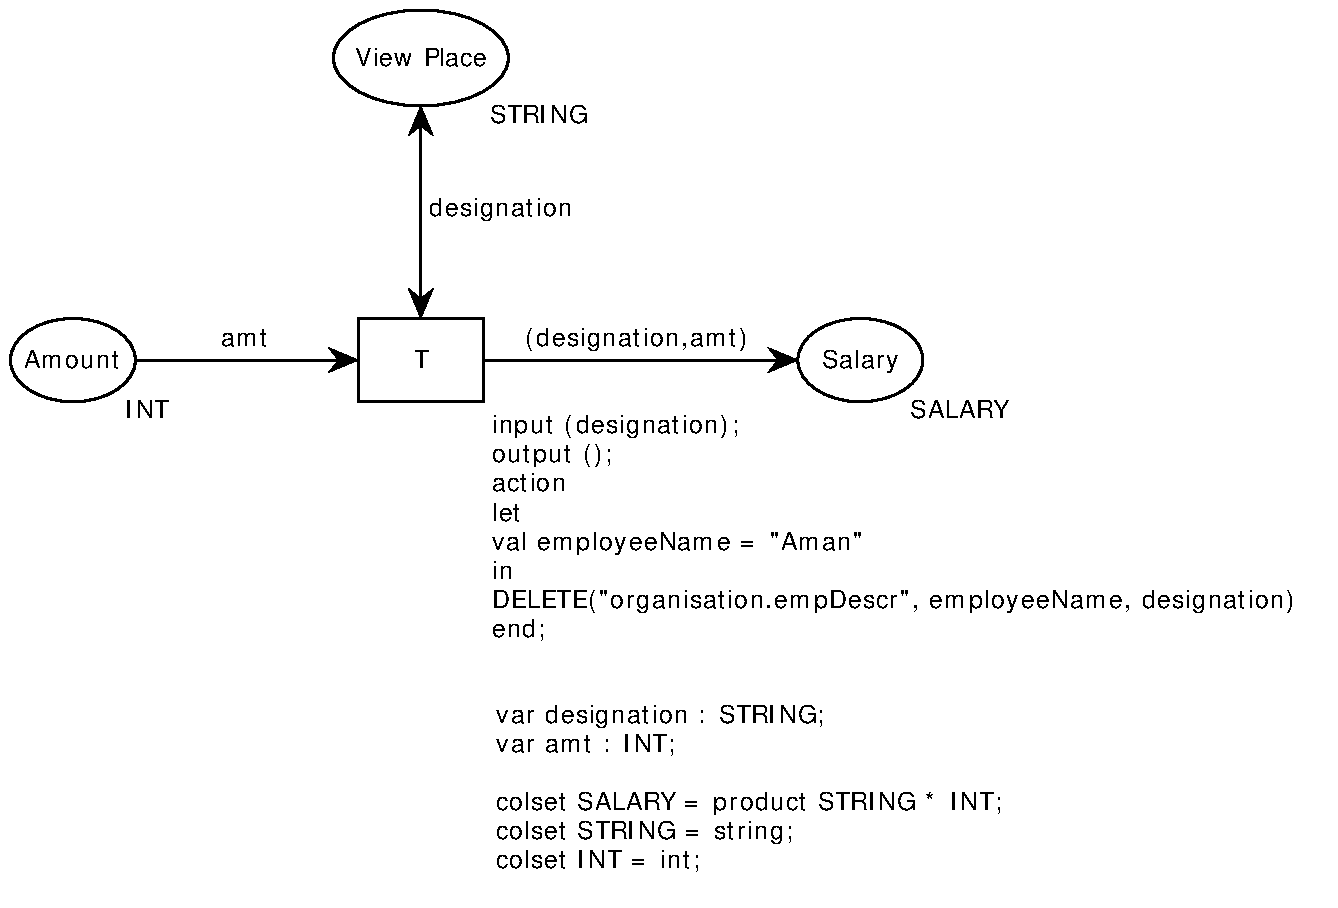
\includegraphics[scale = 0.40]{DBN_SS_Delete_Operation.pdf}
	\caption{DB-nets: delete operation}
	\label{fig:DBN_SS_Delete_Operation}
\end{figure}
\begin{figure}[!htbp]
	\centering
	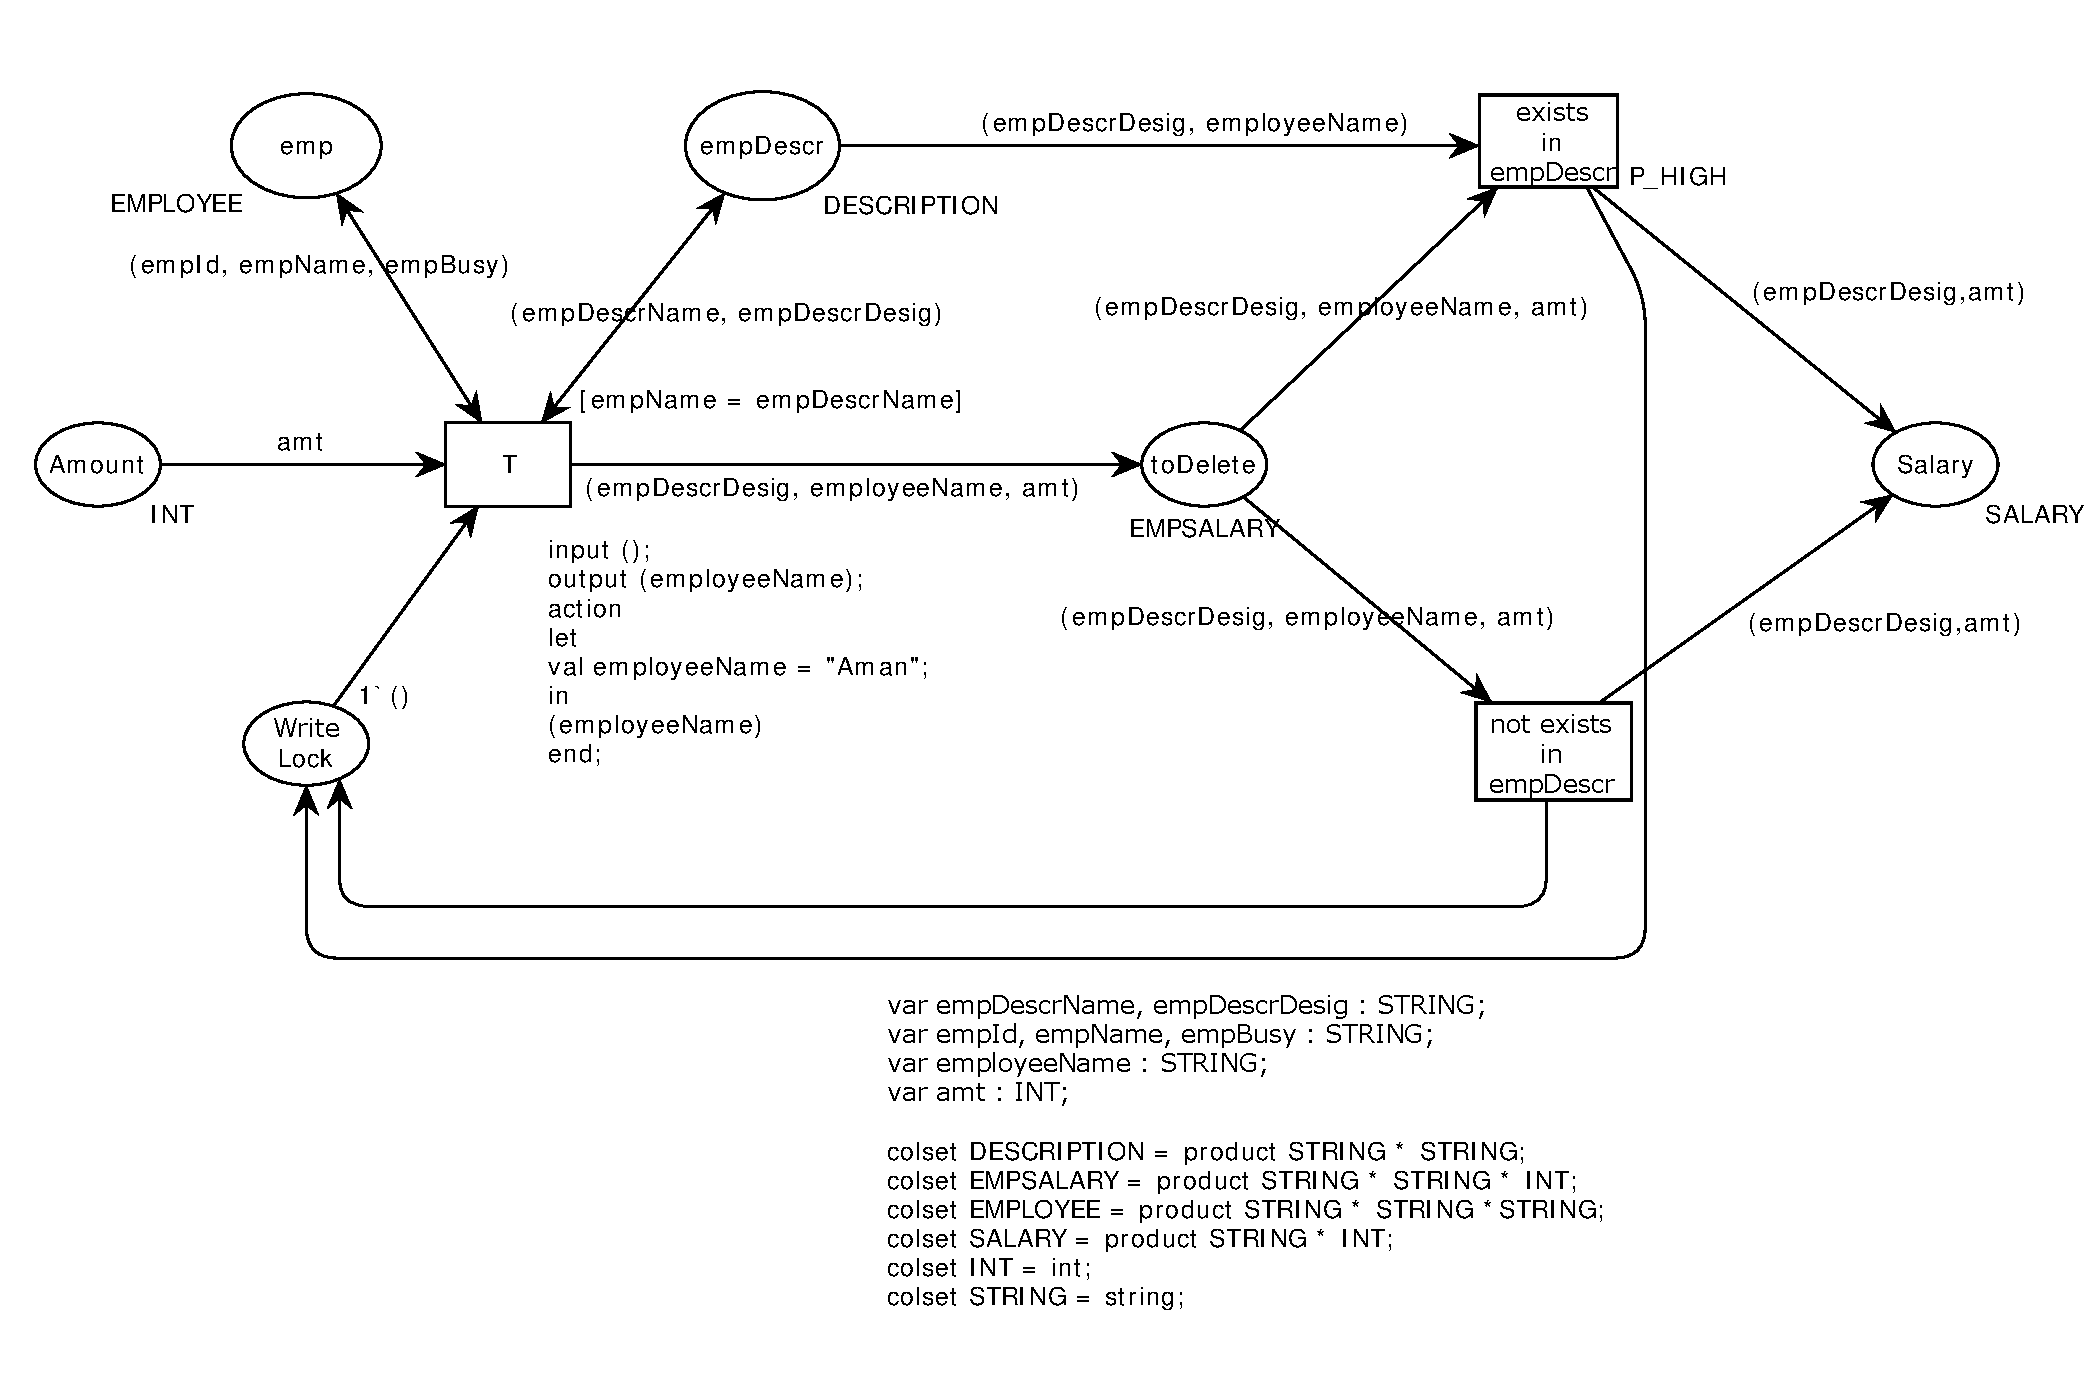
\includegraphics[scale = 0.40]{DBN_SS_Delete_Operation_Relational_Place.pdf}
	\caption{DB-nets: modelling delete operation using relational places}
	\label{fig:DBN_SS_Delete_Operation_Relational_Place}
\end{figure}
}}

\subparagraph*{\textnormal{For $\mathit{UPDATE}$ operation, we can model it using the transformation of DELETE and ADD operations. For update, we assume the case that when an update operation is performed, it should always preserve set semantics.}}

\begin{comment}
 For example, in Figure \ref{fig:DBN_SS_Update_Operation}, we perform an update operation on the relational schema $\mathit{empDescr}$ which updates the given designation to a new designation. The corresponding update operation can be modelled using relational places as shown in Figure \ref{fig:DBN_SS_Update_Operation_Relational_Place}. Here we assume that the tuple to be updated is already present in the relational place and after the update operation the set semantics is preserved at the relational place.}}
	
\begin{figure}[!htbp]
	\centering
	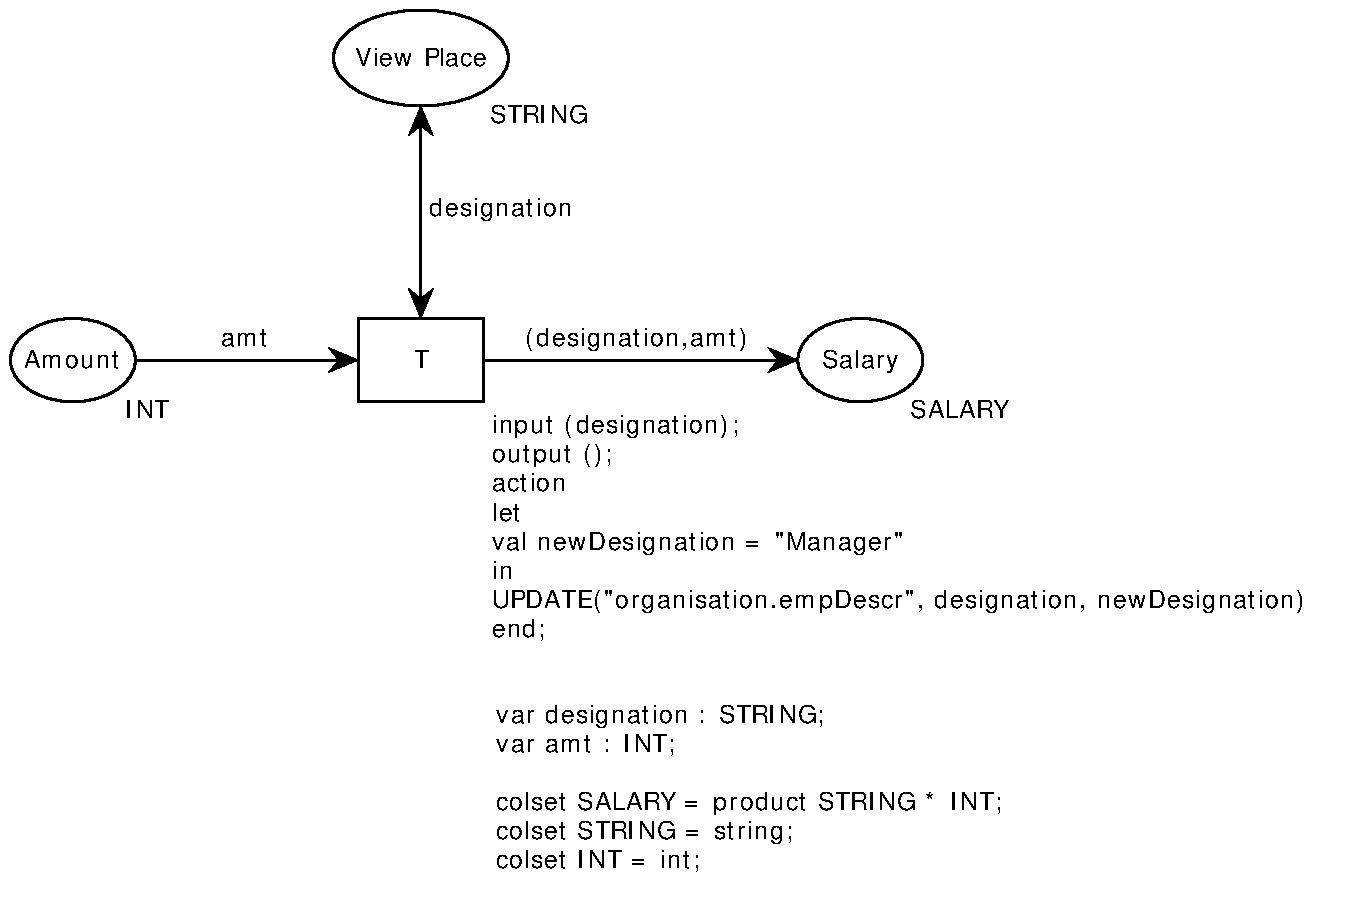
\includegraphics[scale = 0.40]{DBN_SS_Update_Operation.pdf}
	\caption{DB-nets: update operation}
	\label{fig:DBN_SS_Update_Operation}
\end{figure}

\begin{figure}[!htbp]
	\centering
	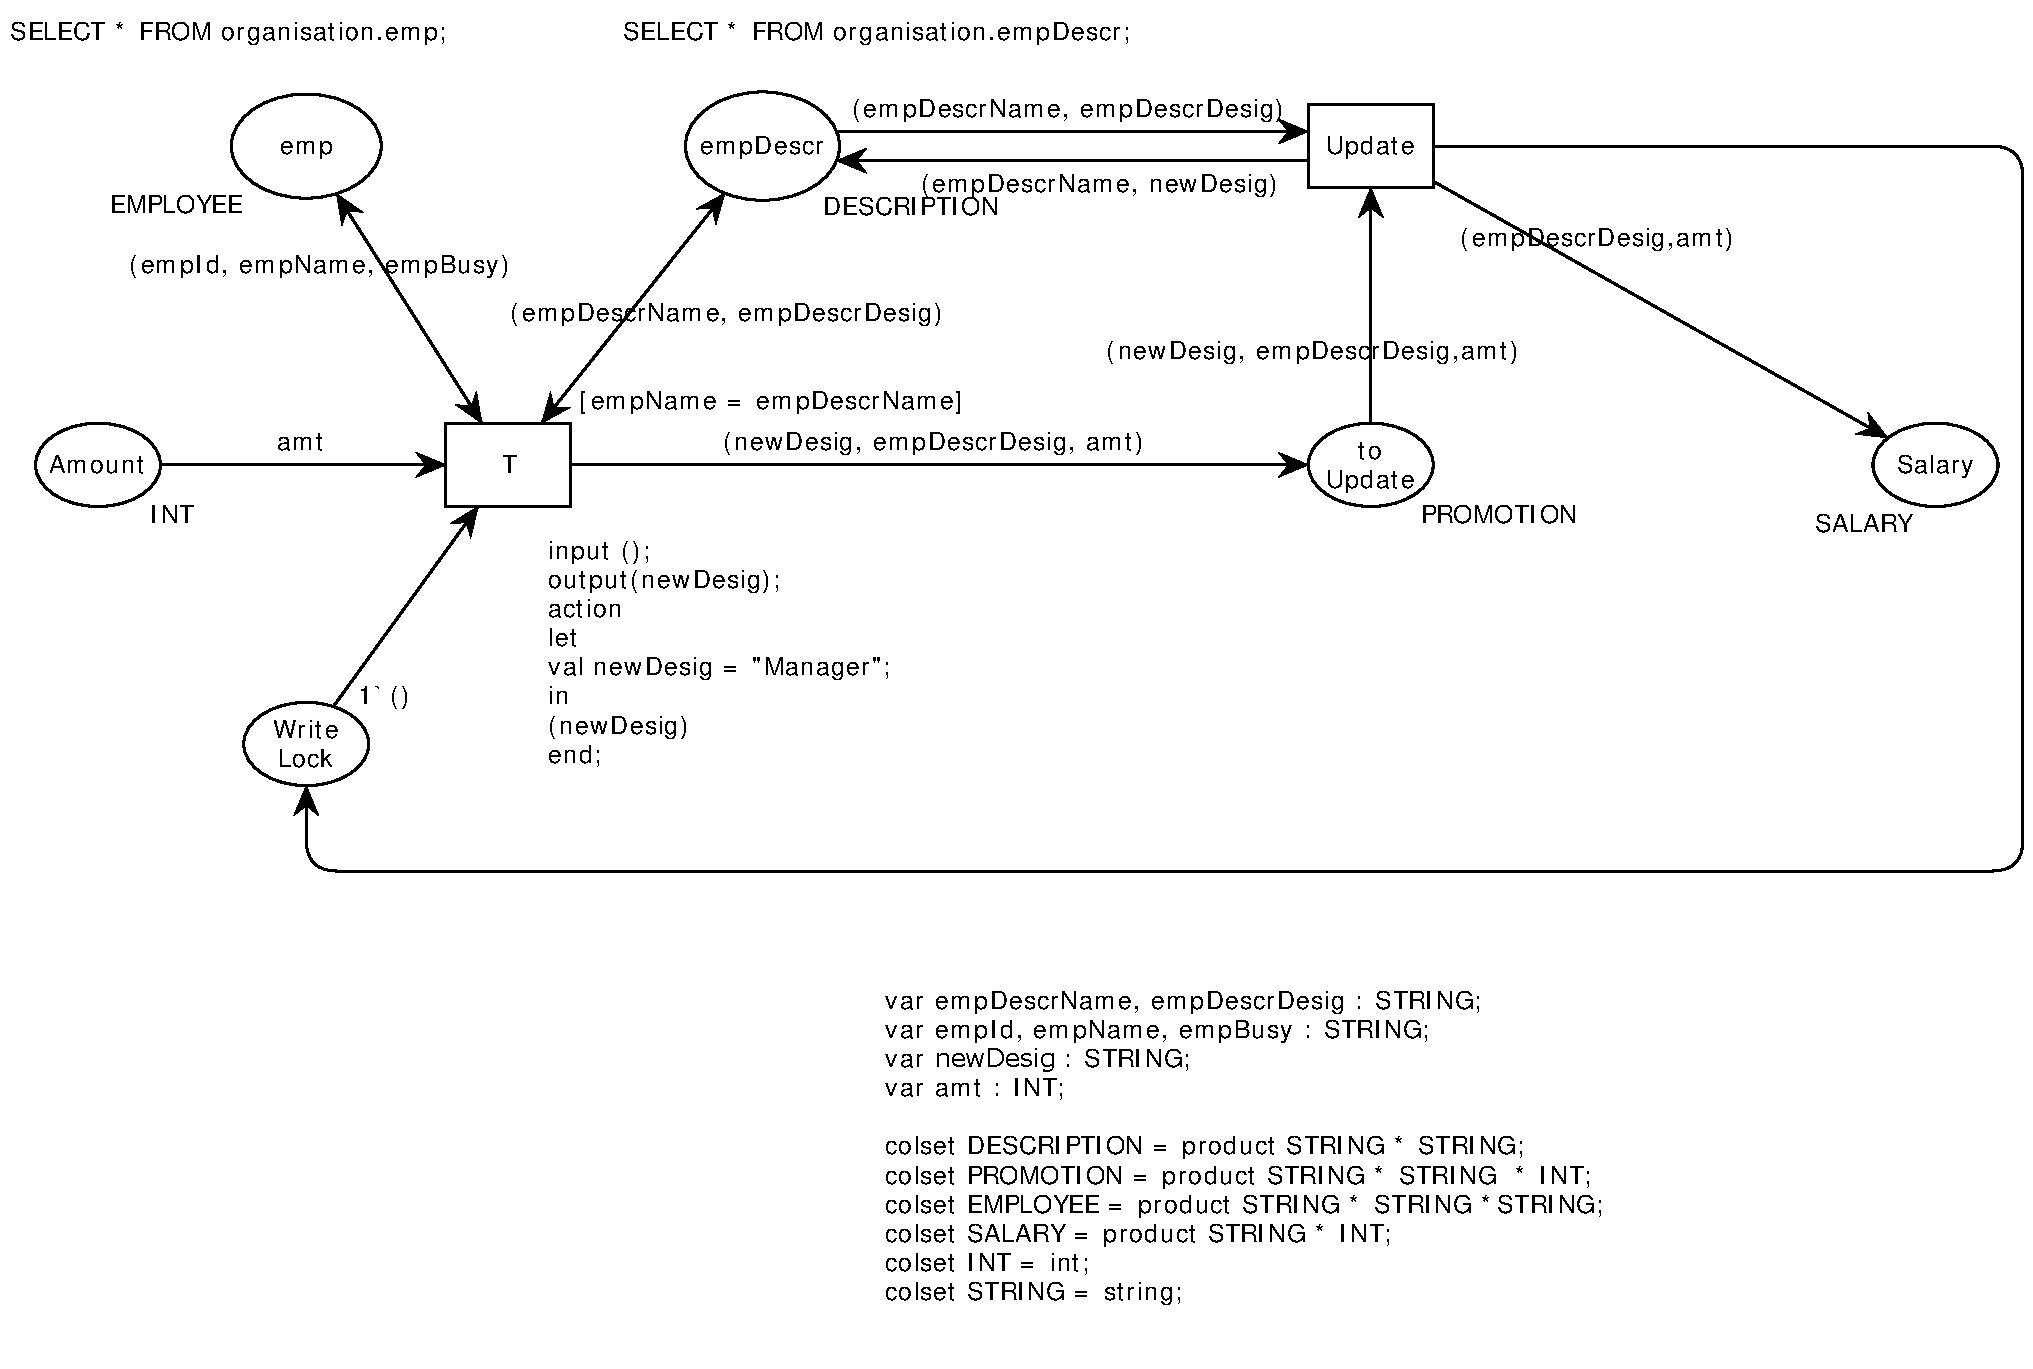
\includegraphics[scale = 0.40]{DBN_SS_Update_Operation_Relational_Place.pdf}
	\caption{DB-nets: modelling update operation using relational places}
	\label{fig:DBN_SS_Update_Operation_Relational_Place}
\end{figure}

\subparagraph*{\textnormal{Note that the $\mathit{READ}$ operation in DB-nets is modelled using view places. View places give us the partial information from the database instance whereas using relational places we represent the entire database instance. We can calculate the partial information (shown by view place) from the relational places and hence we do not need to explicitly model the read operation.}}
\end{comment}

\subparagraph*{\textnormal{In Figure \ref{fig:DBN_SS_Multi_Operations}, we have multiple operations defined in the action transition $\mathit{T}$. The order of execution of these operations are important and the \textit{delete} operation should be performed before the \textit{add} operation. While transforming the DB-net, we model these operations in sequential manner and after performing the last operation we finally return the write lock. The transformation of the DB-net (see Figure \ref{fig:DBN_SS_Multi_Operations}) is shown in Figure \ref{fig:DBN_SS_Multi_Operations_Relational_Places}. Delete operations are performed before add operations, so as to properly reconstruct the semantics of actions in DB-nets. Here, we sequentially perform delete and add operations and the intermediate result (after performing each operation) is propagated into the transformed net. For example, we first perform the delete operation, where we check if the entry exists in the relational place $\mathit{empDescr}$. If the corresponding entry exists in the relational place, then we delete the entry, else we simply propagate the intermediate result to the place $\mathit{toAdd}$. Similarly, for add operation, if the entry exists in the relational place, then we do not add the entry, else we add the entry and propagate the result to the place $\mathit{Salary}$. Since, the order of execution of \textit{delete} and \textit{add} operation is important, we serialize them in our net and return the write lock only when all the operations attached to the transition $\mathit{T}$ is carried out.}}

\begin{figure}[!htbp]
	\centering
	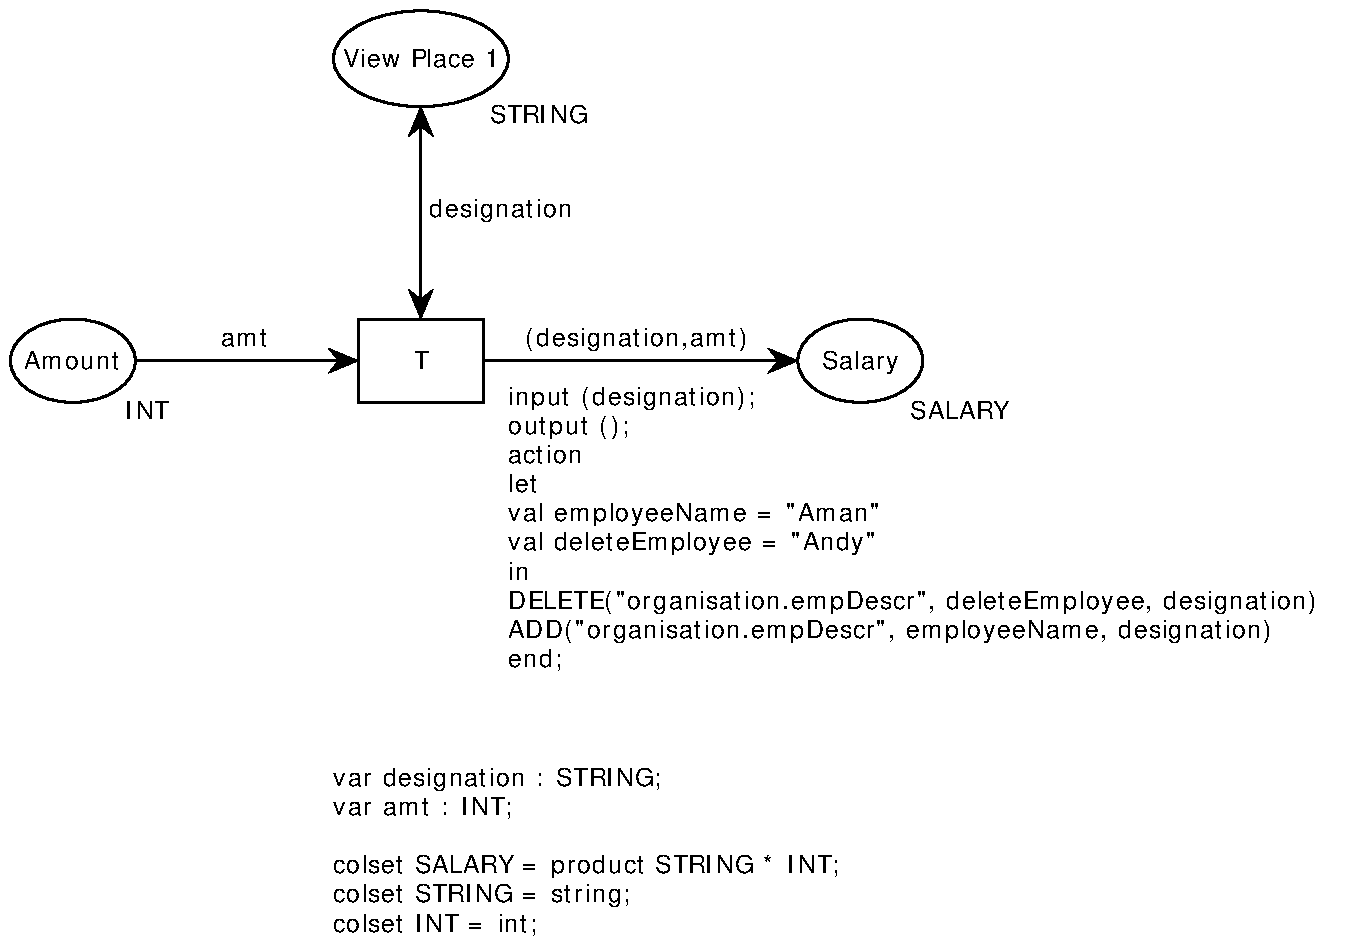
\includegraphics[scale = 0.40]{DBN_SS_Multi_Operations.pdf}
	\caption{DB-nets: action containing multiple operations}
	\label{fig:DBN_SS_Multi_Operations}
\end{figure}

\begin{sidewaysfigure}[!htbp]
\centering
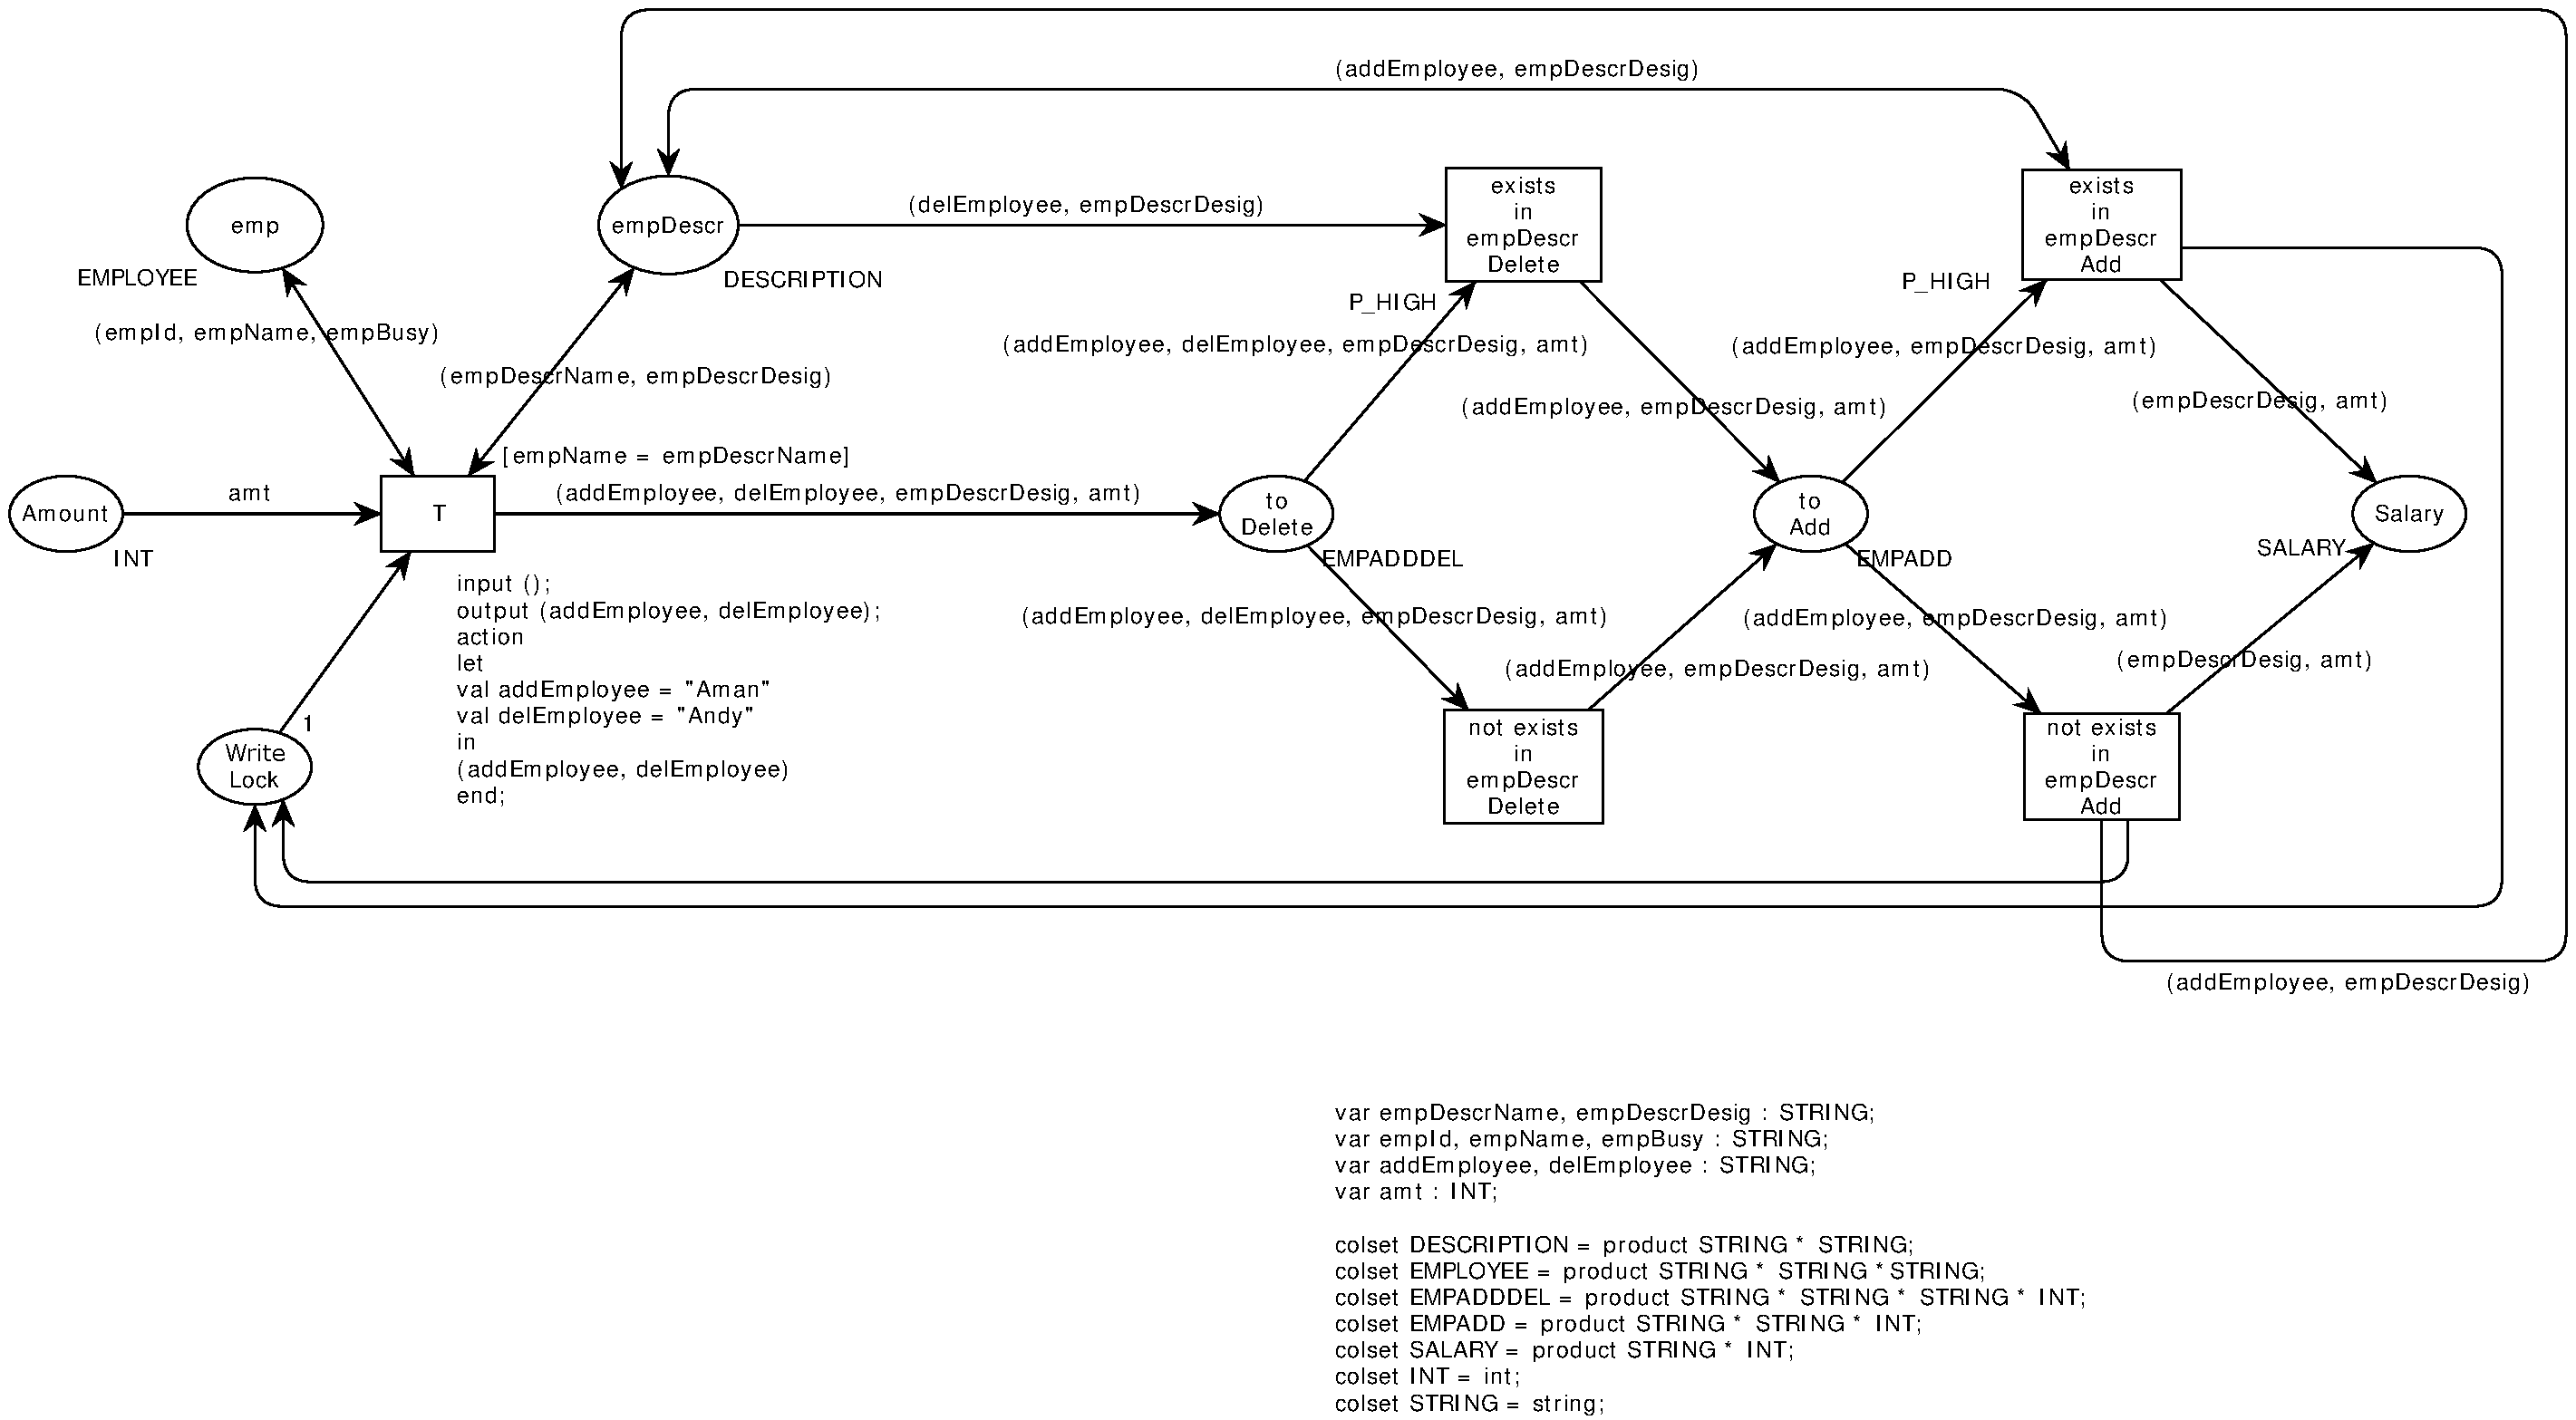
\includegraphics[scale = 0.40]{DBN_SS_Multi_Operations_Relational_Places.pdf}
\caption{DB-nets: modelling all operations sequentially using relational places}
\label{fig:DBN_SS_Multi_Operations_Relational_Places}
\end{sidewaysfigure}

\subparagraph*{\textnormal{Let us incorporate the above mentioned modelling guidelines to model our taxi booking example shown in Figure \ref{fig:DBN_SS_Faulty_Net}. We model the net using relational places as shown in Figure \ref{fig:DBN_SS_Taxi_Booking_model}. Note that the relational place $\mathit{Taxi}$ is populated with three tokens where only the taxi with taxi id = 49209 is free. The guard of the transition $\mathit{Serve Booking}$ makes sure that only free taxi is read from the relational place. The state space calculated by the CPN Tools for this model is shown in Figure \ref{fig:DBN_SS_Correct_CPN_Tools}. Although, due to the presence the additional places and transitions the state space for this model has more nodes as compared the expected state space model (see Figure \ref{fig:DBN_SS_Expected_SS}), however the places of interest show correct markings.
\begin{figure}[!htbp]
	\centering
	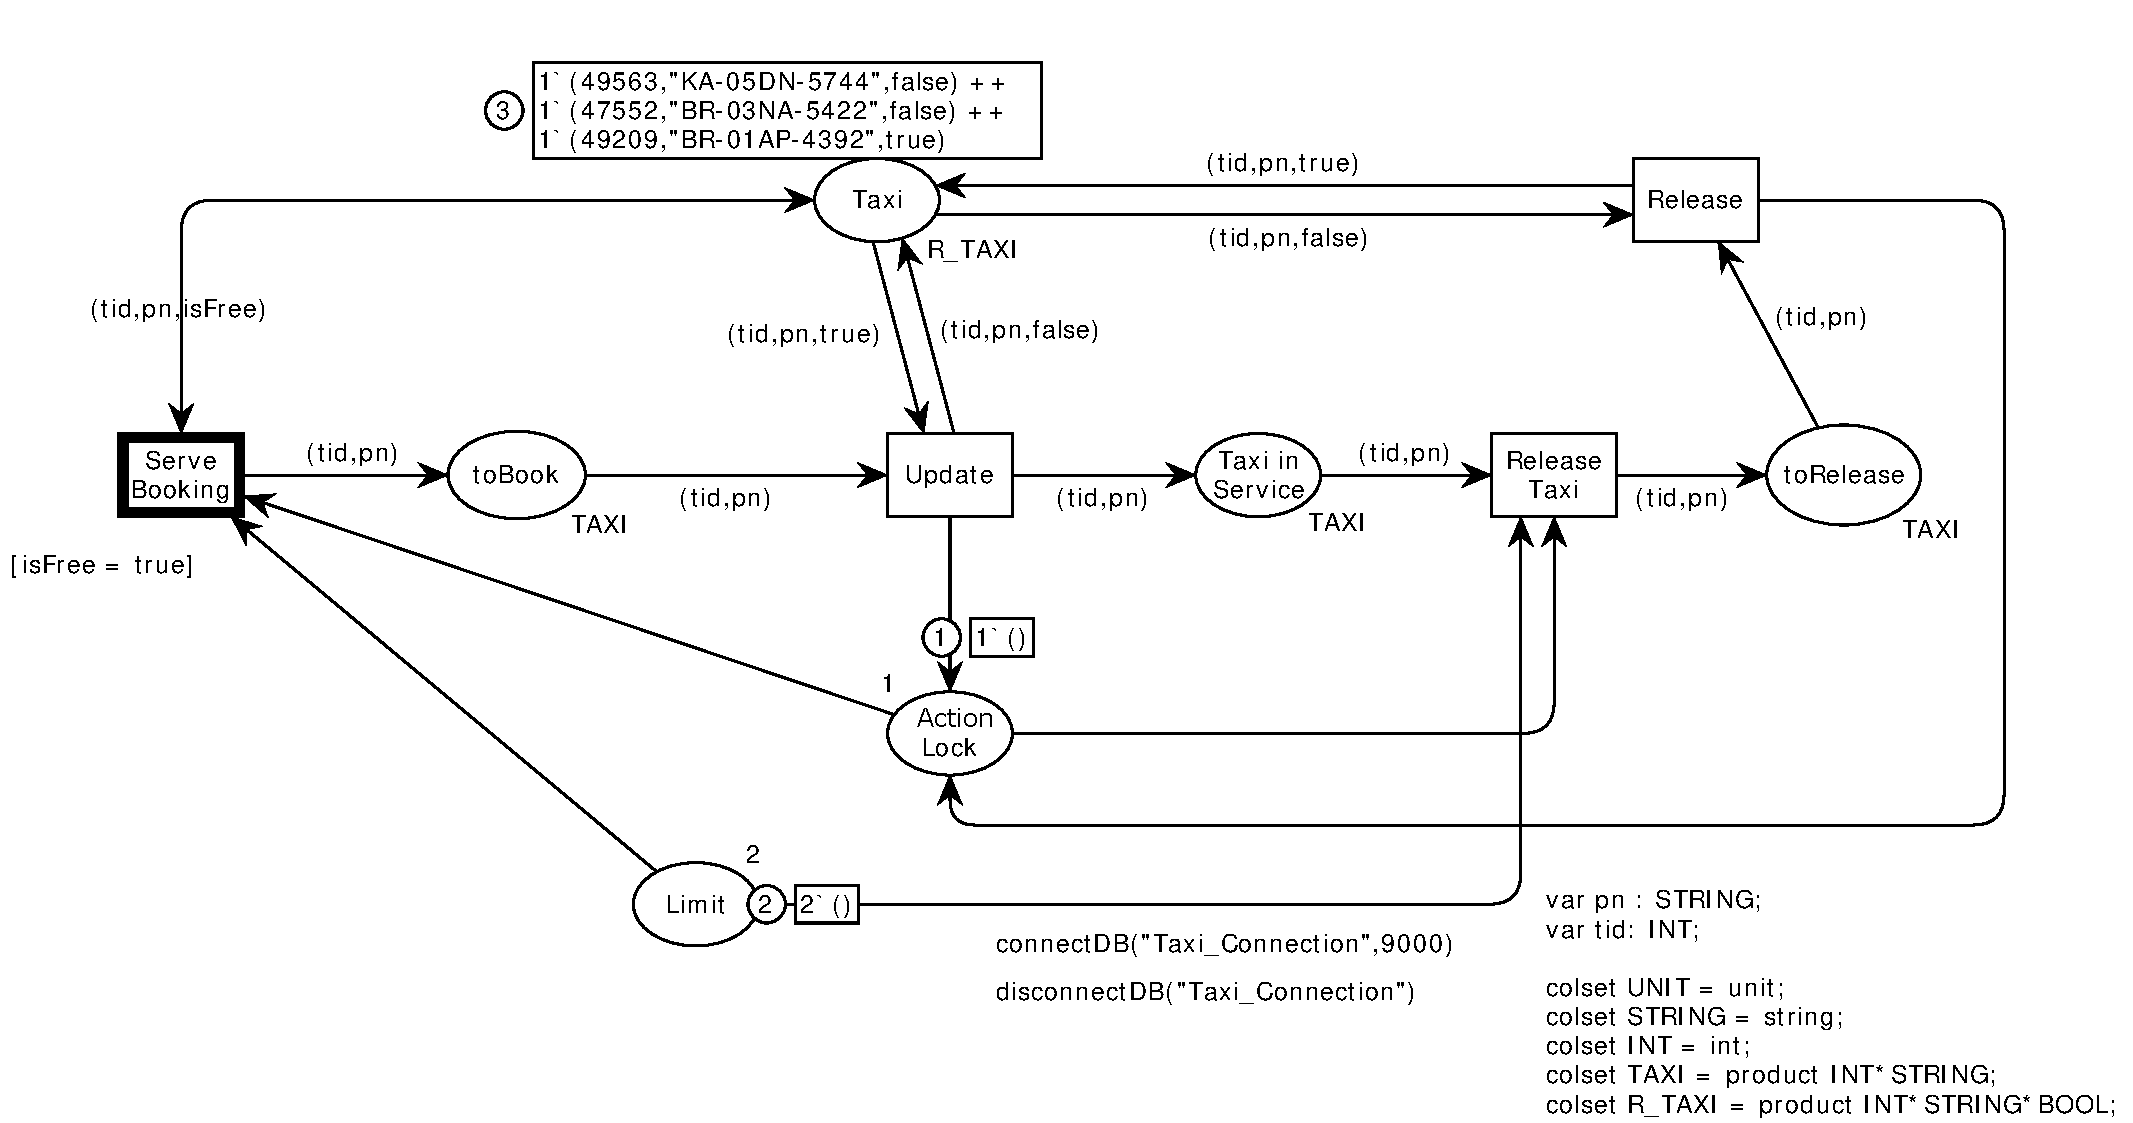
\includegraphics[scale = 0.40]{DBN_SS_Taxi_Booking_model.pdf}
	\caption{Taxi Booking : Transformed net using relational places}
	\label{fig:DBN_SS_Taxi_Booking_model}
\end{figure}
}}

\subparagraph*{\textnormal{Notice that, due to the elimination of view places, the introduction of relational places, and the reconstruction of the semantics of actions via sequences of non-interruptible transitions, the resulting state space does not exactly correspond to the one induced by the original db-net. However, the two state spaces exactly correspond to each other when only focusing on control places and the reachability of their corresponding markings.}}

\begin{figure}[!htbp]
	\centering
	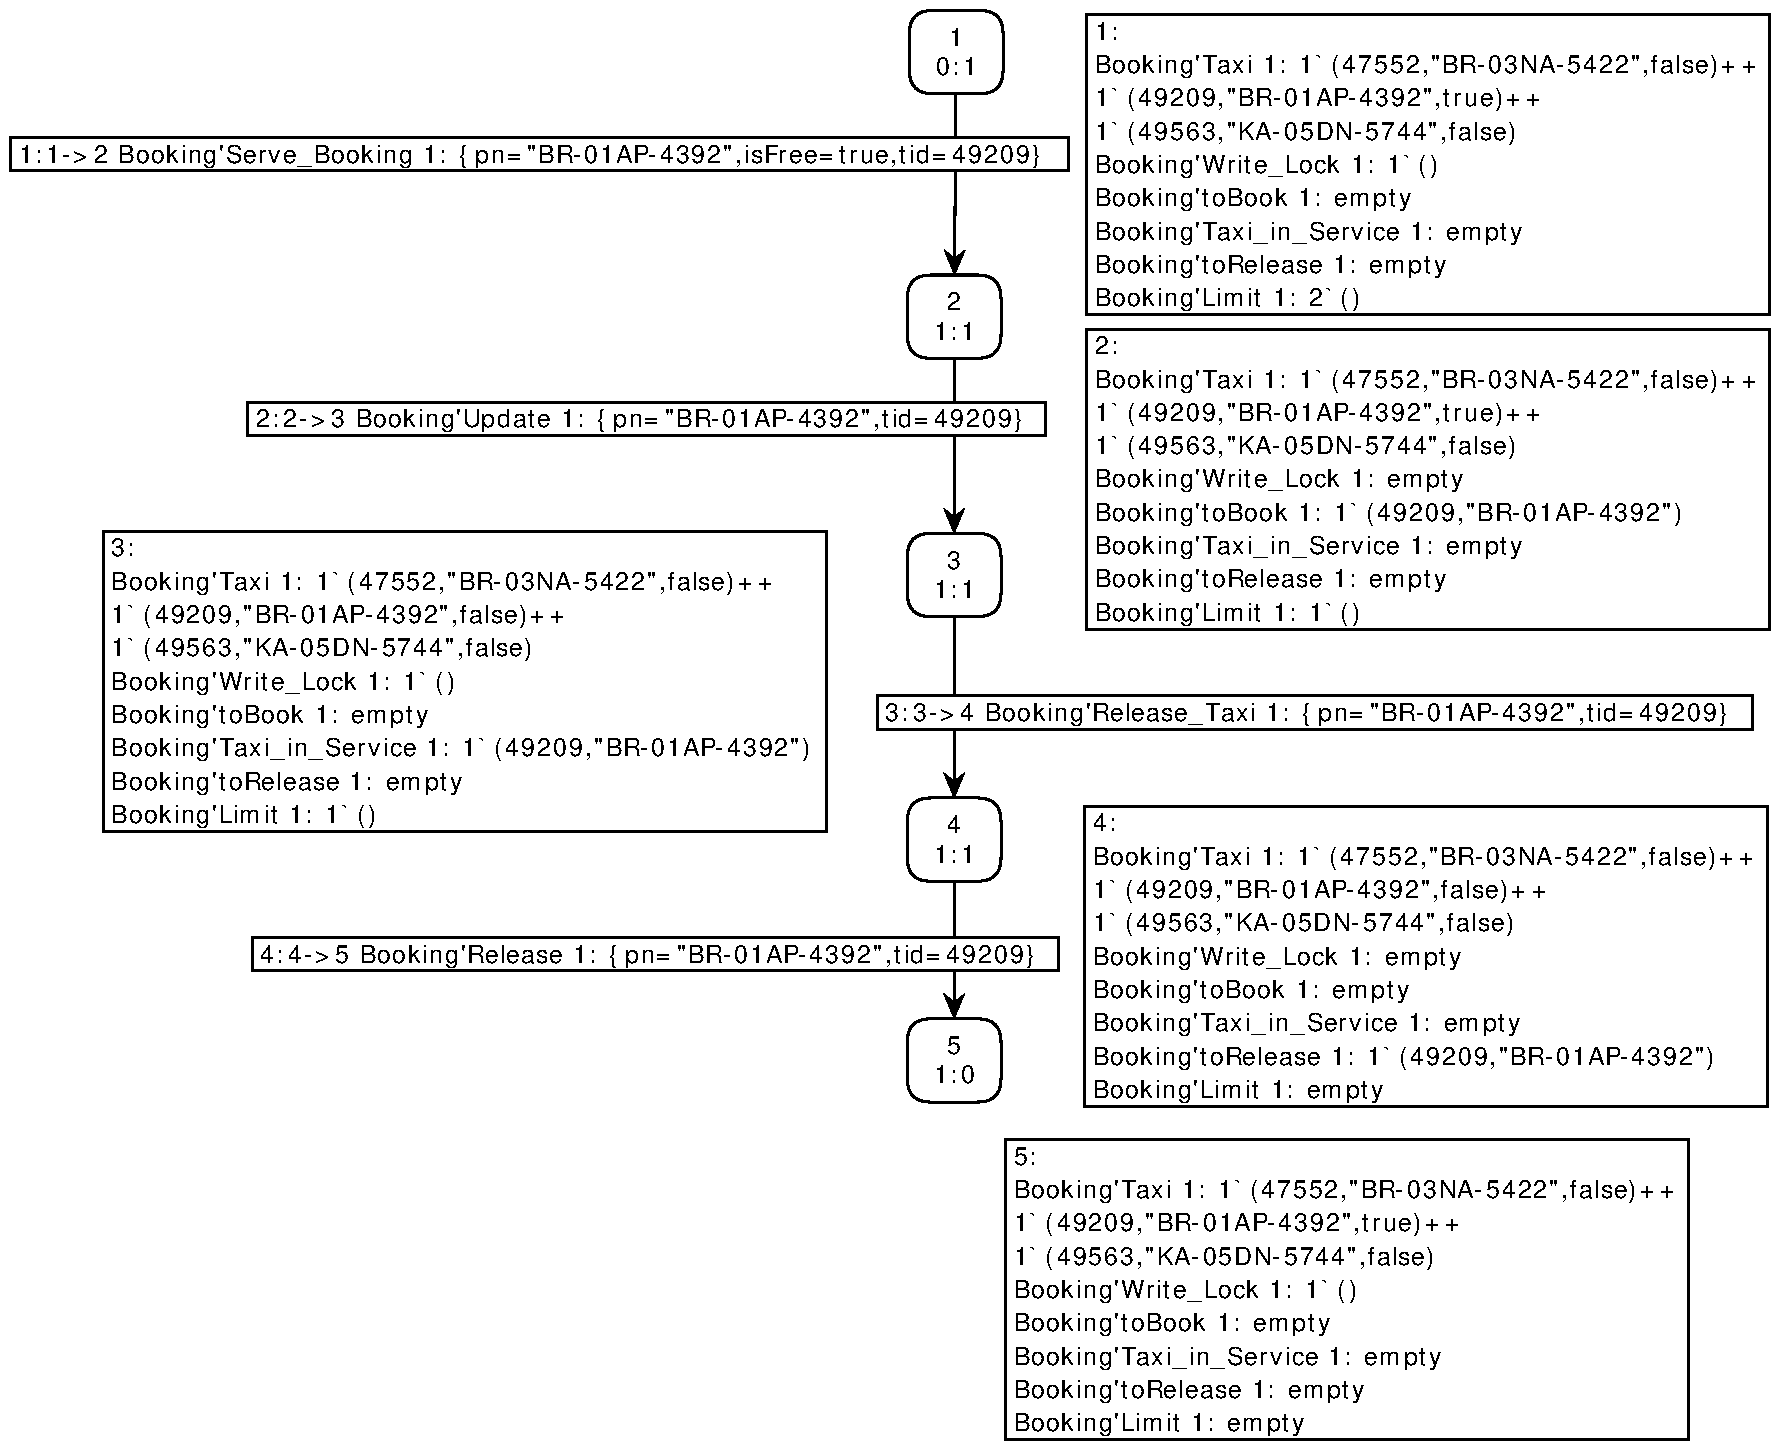
\includegraphics[scale = 0.40]{DBN_SS_Correct_CPN_Tools.pdf}
	\caption{Calculated state space for the model (in Figure \ref{fig:DBN_SS_Taxi_Booking_model}) using state space tool}
	\label{fig:DBN_SS_Correct_CPN_Tools}
\end{figure}



